\documentclass{ctexart}

\usepackage{ctex}
\usepackage{tikz}
\usetikzlibrary{calc,positioning,shapes.geometric}
\usepackage{url}
\usepackage{graphicx}
\usepackage{float}
\usepackage{xcolor}
\usepackage{color}
\usepackage{amsmath}
\usepackage{amsthm}
\usepackage{amssymb}
\usepackage{mathrsfs}
\usepackage{caption}
\usepackage{subfigure}
\usepackage{framed}
\usepackage{booktabs}
\usepackage{makecell}
\usepackage{multirow}
\usepackage{geometry}
\usepackage{wrapfig}
\usepackage{abstract}
\usepackage{algorithmicx}
\usepackage[ruled]{algorithm}
\usepackage{algpseudocode}
\usepackage{setspace}
\usepackage{booktabs}
\usepackage{bm}
\usepackage{cite}
\usepackage{array}

\usepackage{textcomp}
\usepackage{listings}

\definecolor{shadecolor}{rgb}{0.93,0.93,0.93}
\usepackage{geometry}
\geometry{right=2.5cm,left=2.5cm}

\newtheorem{theorem}{定理}

\pagenumbering{arabic}

\begin{document}
\begin{sloppypar}
\title{\vspace{-3cm} \textbf{数值分析项目作业三报告}}
\author{刘陈若\;$3200104872$\\信息与计算科学2001}
\date{}

\maketitle

\section{程序编译和运行说明}
本次项目作业采用Makefile文件对编译进行统一管理。具体地,在Makefile所在目录下输入\verb|make run|
即可完成编译,得到\verb|test.cpp|的可执行文件\verb|test|以及报告所需要的程序运行结果。

需要说明三点:
\begin{itemize}
    \item 1.本项目作业使用json file进行参数输入,以\verb|#include <jsoncpp/json/json.h>|的形式被调用,因此在编译时需要保持相应的文件关系;
    \item 2.在使用json file进行参数输入时,部分参数可能需要修改,参数的含义以及具体的修改方式都将在下文中详细给出;
    \item 3.头文件\verb|TI.h|中使用了\verb|C++17|的structure binding,因此您的电脑需要允许Makefile中使用的\verb|-std=c++17|进行编译。
\end{itemize}

\section{程序运行结果及简要分析}

\subsection{程序测试指南}
所有的任务都可以通过调整\verb|test.json|中的参数得到解决,\verb|test.json|中各参数的含义说明如下:
\begin{itemize}
    \item \verb|initial_value|:数值算法初始值。根据项目作业要求,对于第一个轨道,数值算法初始值应设为\verb|[0.994,0.0,0.0,0.0,-2.0015851063790825224,0.0]|;对于第二个轨道,数值算法初始值应设为\verb|[0.879779227778,0.0,0.0,0.0,-0.379677780949,0.0]|;
    \item \verb|one_period_time|:轨道运行周期$T$。根据项目作业要求,对于第一个轨道,轨道运行周期应设为\verb|17.06521656015796|;对于第二个轨道,轨道运行周期应设为\verb|19.140450691377|;
    \item \verb|one_period_step_number|:单周期数值求解步数$n$,即按照time-step size迭代一个周期需要的迭代次数。需要注意两点:\textbf{首先},例如您可以直接输入\verb|[10000]|代表您希望用10000步完成一个周期的迭代。由于计算收敛阶需要,您也可以输入一个向量\verb|[10000,20000,40000,80000]|,程序将按顺序依次完成对应步数的迭代,并且给出收敛阶。由于在计算收敛阶时我们是取以2为底的对数,因此请确保在向量中每一个元素都是前一个的两倍。\textbf{其次},对于Fehlberg 4(5) embedded RK method和Dormand-Prince 5(4) embedded RK method,由于其是变步长的,因此对于这两个方法我们将把您输入的单周期数值求解步数转化成time-step size并作为初值;
    \item \verb|method|:数值求解算法。根据项目作业要求,对于课本中的八个数值求解算法,
    按从上至下的顺序应依次输入\verb|"Adams_Bashforth"|,\verb|"Adams_Moulton"|,\verb|"Backward_differentiation"|,\verb|"Classical_RK"|,\verb|"explicit_SDIRK"|,\verb|"Gauss_Legendre_RK"|,\verb|"Fehlberg_embedded_RK"|,\verb|"Dormand_Prince_embedded_RK"|;
    \item \verb|order|:算法精度阶数$p$。根据项目作业要求,对于\verb|"Adams_Bashforth"|,精度阶数应取1,2,3,4;对于\verb|"Adams_Moulton"|,精度阶数应取2,3,4,5;对于\verb|"Backward_differentiation"|,精度阶数应取1,2,3,4;对于\verb|"Classical_RK"|,精度阶数应取4;对于\verb|"explicit_SDIRK"|,精度阶数应取4;对于\verb|"Gauss_Legendre_RK"|,精度阶数应取2,4,6(对应s=1,2,3);对于\verb|"Fehlberg_embedded_RK"|,精度阶数应取4(对应4(5));对于\verb|"Dormand_Prince_embedded_RK"|,精度阶数应取5(对应5(4));
    \item \verb|if_Richardson|:是否需要Richardson外插定阶。如输入\verb|"yes"|,则将使用Richardson外插给出算法收敛阶估计;如输入\verb|"no"|,则将不使用Richardson外插。
\end{itemize}


\subsection{轨道一结果展示}
根据项目要求,在这个部分,我对八个数值算法分别对八个轨道所有要求的精度$p$进行数值测试,并给出如下结果:
\begin{itemize}
    \item 1.\textbf{数值结果图像}。我将设置合适的单周期数值求解步数,绘制一幅$u_1$,$u_2$较为精确的图像作为直观展示;
    \item 2.\textbf{不同单周期数值求解步数下的误差}。这里的误差指的是运行一个周期的数值结果和初始值的差的绝对值。我将展示$u_1$到$u_6$每一个分量的绝对误差;
    \item 3.\textbf{算法的收敛阶计算}。根据得到的绝对误差,对于六个分量分别求前后两项的比值,然后取以2为底的对数得到收敛阶,并且给出其平均数作为平均收敛阶。需要注意三点:
\begin{itemize}
    \item 首先,对于一个$p$阶精度的算法,one-step error为$\Theta(k^{p+1})$,而对于一个周期的数值求解步数为$\frac{T}{k}$,因此在运行一个周期之后的误差应是$\Theta(k^{p+1}) \times \frac{T}{k} = O(k^p)$的。所以对于一个$p$阶精度的算法,我们可以期望当$k$足够小时收敛阶应当为$p$;
    \item 其次,我们对每一个分量都计算收敛阶,而不是利用范数计算,这样的结果是合理且更加精确的。这是因为根据one-step error的定义,对于向量函数的每一个维度都应该按照相同的收敛阶收敛,如果用范数计算(如无穷范数)则会丢掉那些量级较小的分量的收敛信息;
    \item 第三,由于$u_3$和$u_6$分量恒为0,因此不纳入收敛阶计算的范围之内;
\end{itemize}
    \item 4.\textbf{算法CPU运行时间}。我将给出算法求解过程中的运行时间对比;
    \item 5.\textbf{算法最大可行步长 $n_{\max}$}。我将给出一个时间步长界,使得当步长再增大之后算法得到的图像就会产生肉眼可见的偏移。这里我们认为当$u_1$或者$u_2$的计算解和真实值的绝对误差达到$5 \times 10^{-2}$时,图像的偏移就会被肉眼观察到。
\end{itemize}
并且在本节的最后(2.2.9节),我将完成作业要求的最后部分,绘制并且比较Euler's method, classical RK method, Dormand-Prince 5(4) embedded RK method的相关图像和运行时间等。

\subsubsection{Adams-Bashforth methods}
我们根据\textbf{Definition 11.83}和\textbf{Definition 11.84}编写了Adams-Bashforth算法,需要注意的是对于$p > 1$的情况,我们需要用合适的方法获得足够的初始值进行迭代,因此,为了保证初始值的精度,我们采用经典四阶RK获得足够的初始值。(对于轨道二也是如此,因此在2.3节中不再赘述)

$\bullet \;$ $p = 1$

首先,设置单周期数值求解步数$n = 8 \times 10^6$(\textbf{关于项目作业要求的24000 steps的图像及其运行时间分析请见2.2.9节}),绘制轨道一图像(作为直观展示)如下。此时轨道基本上没有肉眼可见的偏离,这是算法正确性的体现。
\begin{figure}[H]
\centering
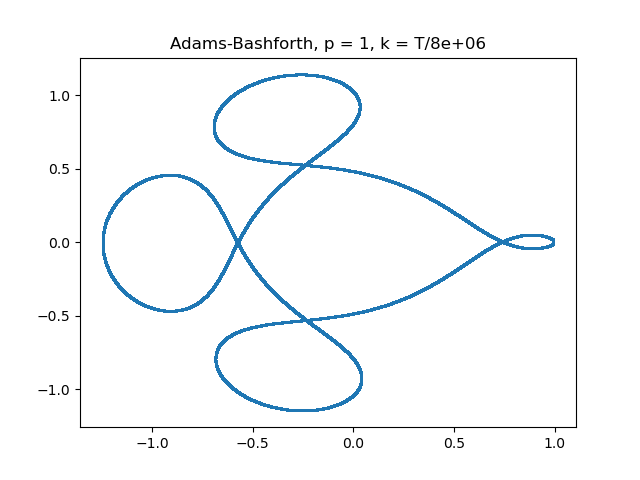
\includegraphics[scale = 0.45]{./report_src/Figure_1.png}
\end{figure}
其次,设置单周期数值求解步数分别为$n = 4 \times 10^6,8 \times 10^6,1.6 \times 10^7, 3.2 \times 10^7$(为了能得到相对准确的收敛阶,我们选取相对较大的$n$),得到$u_1$至$u_6$分量和初始值的绝对误差、对应算法收敛阶以及CPU time如下表所示:

\begin{table}[H]
\renewcommand{\arraystretch}{1.5}
\begin{center}
\begin{tabular}{c|c@{\hspace{0.2cm}}c
|c@{\hspace{0.2cm}}c|c@{\hspace{0.2cm}}c|c@{\hspace{0.2cm}}c}
  \hline
  \multirow{2}{*}{$\backslash$ \textbf{n}} & \multicolumn{2}{c|}{$4 \times 10^6$} & \multicolumn{2}{c|}{$8 \times 10^6$} & \multicolumn{2}{c|}{$1.6 \times 10^7$} & \multicolumn{2}{c}{$3.2 \times 10^7$} \\
  \cline{2-9}
  & 绝对误差&收敛阶 & 绝对误差 &收敛阶& 绝对误差 & 收敛阶 &绝对误差& 收敛阶 \\
  \hline
  $u_1$ & 1.071e-03 &$\backslash$  & 1.139e-05 &6.555 & 5.328e-05 &-1.548 & 5.631e-04 &-0.080 \\
$u_2$ & 2.564e-02 &$\backslash$  & 1.397e-02 &0.876 & 7.572e-03 &0.883 & 3.982e-03 &0.927 \\
$u_3$ & 0 &$\backslash$  & 0 &$\backslash$  & 0 &$\backslash$  & 0 &$\backslash$  \\
$u_4$ & 6.841e-01 &$\backslash$  & 7.350e-01 &-0.104 & 6.615e-01 &0.152 & 4.757e-01 &0.476 \\
$u_5$ & 1.248e+00 &$\backslash$  & 9.250e-01 &0.432 & 5.631e-01 &0.716 & 2.779e-01 &1.019 \\
$u_6$ & 0 &$\backslash$  & 0 &$\backslash$  & 0 &$\backslash$  & 0 &$\backslash$  \\
\hline
平均收敛阶 & \multicolumn{2}{c|}{ $\backslash$ } & \multicolumn{2}{c|}{1.94} & \multicolumn{2}{c|}{0.05} & \multicolumn{2}{c}{0.59} \\
\hline
CPU time(ms) & \multicolumn{2}{c|}{967} & \multicolumn{2}{c|}{1719} & \multicolumn{2}{c|}{3407} & \multicolumn{2}{c}{6743} \\
\hline

\end{tabular}
\end{center}
\end{table}
从中可以看出,算法的收敛阶并不固定,我们在此进行如实汇报,但是正如您将在2.3节中所看到的,\textbf{对于轨道二该方法的收敛阶是准确的!关于其在轨道一的不稳定性的可能原因请见2.2.10节}。CPU time与步数$n$基本成正比关系。

此外,以$10^4$为单位不断改变步数$n$,得到当$n = 1.90 \times 10^6$时,$u_1$和$u_2$的误差较大值为$4.98 \times 10^{-2}$,最接近给定阈值$5 \times 10^{-2}$,从而产生肉眼可见的偏离如下(对比上文中的较精确图像):
\begin{figure}[H]
\centering
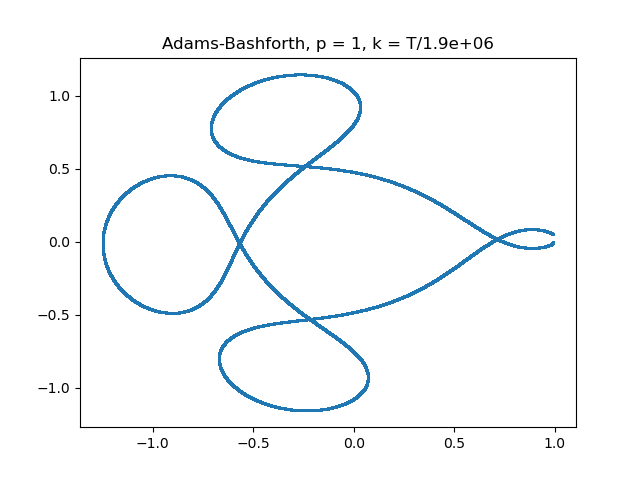
\includegraphics[scale = 0.45]{./report_src/Figure_2.png}
\end{figure}
因此我们得到,算法最大可行步长约为$n_{\max} = 1.90 \times 10^6$。

$\bullet \;$ $p = 2$

首先,设置单周期数值求解步数$n = 2 \times 10^6$,绘制轨道一图像(作为直观展示)如下。此时轨道基本上没有肉眼可见的偏离,这是算法正确性的体现。
\begin{figure}[H]
\centering
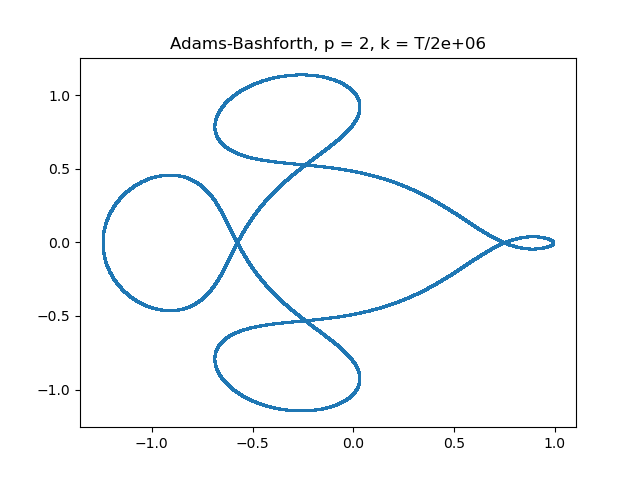
\includegraphics[scale = 0.45]{./report_src/Figure_3.png}
\end{figure}
其次,设置单周期数值求解步数分别为$n = 1 \times 10^6,2 \times 10^6,4 \times 10^6, 8 \times 10^6$(为了能得到相对准确的收敛阶,我们选取相对较大的$n$),得到$u_1$至$u_6$分量和初始值的绝对误差、对应算法收敛阶以及CPU time如下表所示:

\begin{table}[H]
\renewcommand{\arraystretch}{1.5}
\begin{center}
\begin{tabular}{c|c@{\hspace{0.2cm}}c
|c@{\hspace{0.2cm}}c|c@{\hspace{0.2cm}}c|c@{\hspace{0.2cm}}c}
  \hline
  \multirow{2}{*}{$\backslash$ \textbf{n}} & \multicolumn{2}{c|}{$1 \times 10^6$} & \multicolumn{2}{c|}{$2 \times 10^6$} & \multicolumn{2}{c|}{$4 \times 10^6$} & \multicolumn{2}{c}{$8 \times 10^6$} \\
  \cline{2-9}
  & 绝对误差&收敛阶 & 绝对误差 &收敛阶& 绝对误差 & 收敛阶 &绝对误差& 收敛阶 \\
  \hline
  $u_1$ & 3.516e-04 &$\backslash$  & 8.516e-05 &2.108 & 2.071e-05 &2.040 & 5.144e-06 &2.010 \\
$u_2$ & 1.131e-03 &$\backslash$  & 2.837e-04 &1.996 & 7.097e-05 &1.999 & 1.775e-05 &1.999 \\
$u_3$ & 0 &$\backslash$  & 0 &$\backslash$  & 0 &$\backslash$  & 0 &$\backslash$  \\
$u_4$ & 1.970e-01 &$\backslash$  & 4.695e-02 &2.069 & 1.158e-02 &2.019 & 2.886e-03 &2.005 \\
$u_5$ & 3.945e-02 &$\backslash$  & 1.181e-02 &1.740 & 3.135e-03 &1.914 & 7.951e-04 &1.979 \\
$u_6$ & 0 &$\backslash$  & 0 &$\backslash$  & 0 &$\backslash$  & 0 &$\backslash$  \\
\hline
平均收敛阶 & \multicolumn{2}{c|}{ $\backslash$ } & \multicolumn{2}{c|}{1.97} & \multicolumn{2}{c|}{1.99} & \multicolumn{2}{c}{2.00} \\
\hline
CPU time(ms) & \multicolumn{2}{c|}{329} & \multicolumn{2}{c|}{617} & \multicolumn{2}{c|}{1170} & \multicolumn{2}{c}{2295} \\
\hline

\end{tabular}
\end{center}
\end{table}
从中可以看出,随着$n$的增大,算法的收敛阶稳定在2,从而验证了算法的精度为2;CPU time与步数$n$基本成正比关系。

此外,以$10^3$为单位不断改变步数$n$,得到当$n = 1.08 \times 10^5$时,$u_1$和$u_2$的误差较大值为$4.97 \times 10^{-2}$,最接近给定阈值$5 \times 10^{-2}$,从而产生肉眼可见的偏离如下(对比上文中的较精确图像):
\begin{figure}[H]
\centering
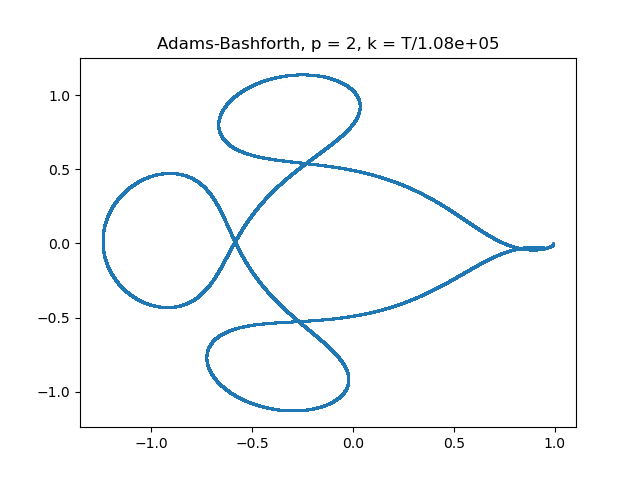
\includegraphics[scale = 0.45]{./report_src/Figure_4.png}
\end{figure}
因此我们得到,算法最大可行步长约为$n_{\max} = 1.08 \times 10^5$,远小于$p=1$时的最大可行步长。

$\bullet \;$ $p = 3$

首先,设置单周期数值求解步数$n = 1 \times 10^5$,绘制轨道一图像(作为直观展示)如下。此时轨道基本上没有肉眼可见的偏离,这是算法正确性的体现。
\begin{figure}[H]
\centering
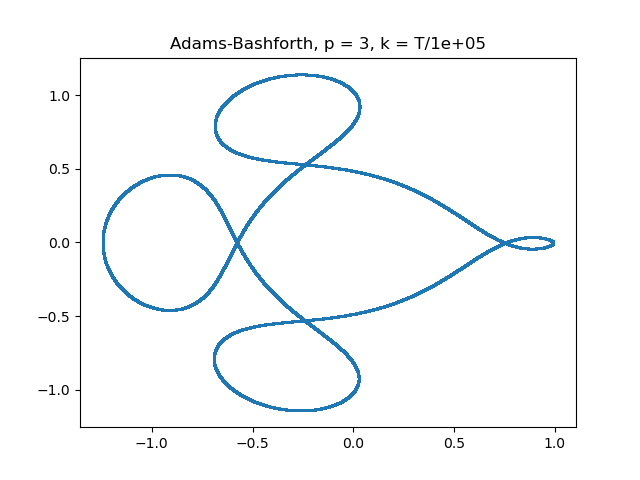
\includegraphics[scale = 0.45]{./report_src/Figure_5.png}
\end{figure}
其次,设置单周期数值求解步数分别为$n = 5 \times 10^5,1 \times 10^6,2 \times 10^6, 4 \times 10^6$(为了能得到相对准确的收敛阶,我们选取相对较大的$n$),得到$u_1$至$u_6$分量和初始值的绝对误差、对应算法收敛阶以及CPU time如下表所示:

\begin{table}[H]
\renewcommand{\arraystretch}{1.5}
\begin{center}
\begin{tabular}{c|c@{\hspace{0.2cm}}c
|c@{\hspace{0.2cm}}c|c@{\hspace{0.2cm}}c|c@{\hspace{0.2cm}}c}
  \hline
  \multirow{2}{*}{$\backslash$ \textbf{n}} & \multicolumn{2}{c|}{$5 \times 10^5$} & \multicolumn{2}{c|}{$1 \times 10^6$} & \multicolumn{2}{c|}{$2 \times 10^6$} & \multicolumn{2}{c}{$4 \times 10^6$} \\
  \cline{2-9}
  & 绝对误差&收敛阶 & 绝对误差 &收敛阶& 绝对误差 & 收敛阶 &绝对误差& 收敛阶 \\
  \hline
  $u_1$ & 1.681e-06 &$\backslash$  & 2.161e-07 &2.959 & 2.740e-08 &2.980 & 3.445e-09 &2.992 \\
$u_2$ & 5.934e-06 &$\backslash$  & 7.618e-07 &2.961 & 9.648e-08 &2.981 & 1.212e-08 &2.992 \\
$u_3$ & 0 &$\backslash$  & 0 &$\backslash$  & 0 &$\backslash$  & 0 &$\backslash$  \\
$u_4$ & 9.637e-04 &$\backslash$  & 1.237e-04 &2.962 & 1.566e-05 &2.981 & 1.969e-06 &2.992 \\
$u_5$ & 2.608e-04 &$\backslash$  & 3.361e-05 &2.956 & 4.262e-06 &2.979 & 5.358e-07 &2.992 \\
$u_6$ & 0 &$\backslash$  & 0 &$\backslash$  & 0 &$\backslash$  & 0 &$\backslash$  \\
\hline
平均收敛阶 & \multicolumn{2}{c|}{ $\backslash$ } & \multicolumn{2}{c|}{2.96} & \multicolumn{2}{c|}{2.98} & \multicolumn{2}{c}{2.99} \\
\hline
CPU time(ms) & \multicolumn{2}{c|}{215} & \multicolumn{2}{c|}{404} & \multicolumn{2}{c|}{779} & \multicolumn{2}{c}{1559} \\
\hline

\end{tabular}
\end{center}
\end{table}
从中可以看出,随着$n$的增大,算法的收敛阶稳定趋向于3,从而验证了算法的精度为3;CPU time与步数$n$基本成正比关系。

此外,以$10^2$为单位不断改变步数$n$,得到当$n = 3.59 \times 10^4$时,$u_1$和$u_2$的误差较大值为$4.96 \times 10^{-2}$,最接近给定阈值$5 \times 10^{-2}$,从而产生肉眼可见的偏离如下(对比上文中的较精确图像):
\begin{figure}[H]
\centering
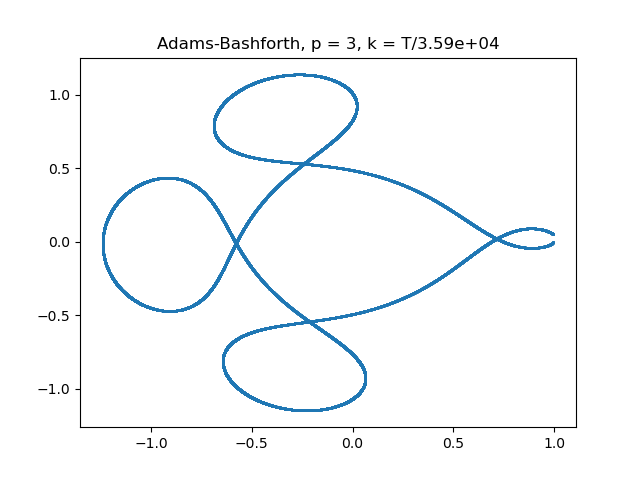
\includegraphics[scale = 0.45]{./report_src/Figure_6.png}
\end{figure}
因此我们得到,算法最大可行步长约为$n_{\max} = 3.59 \times 10^4$,远小于$p=2$时的最大可行步长。

$\bullet \;$ $p = 4$

首先,设置单周期数值求解步数$n = 8 \times 10^4$,绘制轨道一图像(作为直观展示)如下。此时轨道基本上没有肉眼可见的偏离,这是算法正确性的体现。
\begin{figure}[H]
\centering
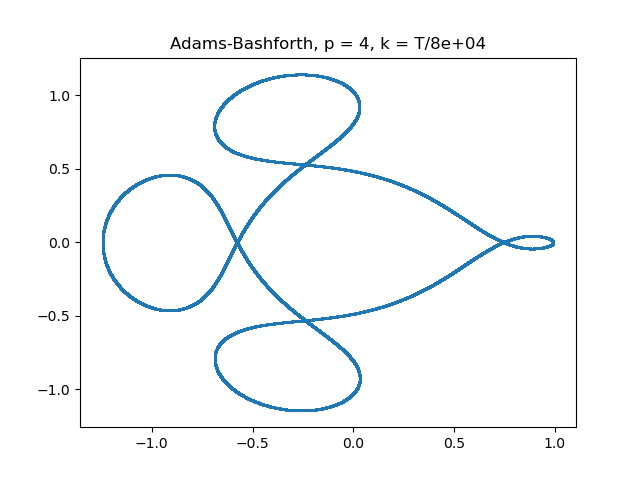
\includegraphics[scale = 0.45]{./report_src/Figure_7.png}
\end{figure}
其次,设置单周期数值求解步数分别为$n = 2 \times 10^5,4 \times 10^5,8 \times 10^5, 1.6 \times 10^6$(为了能得到相对准确的收敛阶,我们选取相对较大的$n$),得到$u_1$至$u_6$分量和初始值的绝对误差、对应算法收敛阶以及CPU time如下表所示:

\begin{table}[H]
\renewcommand{\arraystretch}{1.5}
\begin{center}
\begin{tabular}{c|c@{\hspace{0.2cm}}c
|c@{\hspace{0.2cm}}c|c@{\hspace{0.2cm}}c|c@{\hspace{0.2cm}}c}
  \hline
  \multirow{2}{*}{$\backslash$ \textbf{n}} & \multicolumn{2}{c|}{$2 \times 10^5$} & \multicolumn{2}{c|}{$4 \times 10^5$} & \multicolumn{2}{c|}{$8 \times 10^5$} & \multicolumn{2}{c}{$1.6 \times 10^6$} \\
  \cline{2-9}
  & 绝对误差&收敛阶 & 绝对误差 &收敛阶& 绝对误差 & 收敛阶 &绝对误差& 收敛阶 \\
  \hline
  $u_1$ & 2.975e-05 &$\backslash$  & 1.952e-06 &3.930 & 1.241e-07 &3.975 & 7.821e-09 &3.988 \\
$u_2$ & 1.016e-04 &$\backslash$  & 6.565e-06 &3.952 & 4.166e-07 &3.978 & 2.623e-08 &3.990 \\
$u_3$ & 0 &$\backslash$  & 0 &$\backslash$  & 0 &$\backslash$  & 0 &$\backslash$  \\
$u_4$ & 1.639e-02 &$\backslash$  & 1.067e-03 &3.942 & 6.772e-05 &3.977 & 4.263e-06 &3.989 \\
$u_5$ & 4.807e-03 &$\backslash$  & 3.046e-04 &3.980 & 1.933e-05 &3.978 & 1.217e-06 &3.989 \\
$u_6$ & 0 &$\backslash$  & 0 &$\backslash$  & 0 &$\backslash$  & 0 &$\backslash$  \\
\hline
平均收敛阶 & \multicolumn{2}{c|}{ $\backslash$ } & \multicolumn{2}{c|}{3.95} & \multicolumn{2}{c|}{3.98} & \multicolumn{2}{c}{3.99} \\
\hline
CPU time(ms) & \multicolumn{2}{c|}{134} & \multicolumn{2}{c|}{248} & \multicolumn{2}{c|}{463} & \multicolumn{2}{c}{789} \\
\hline

\end{tabular}
\end{center}
\end{table}
从中可以看出,随着$n$的增大,算法的收敛阶稳定趋向于4,从而验证了算法的精度为4;CPU time与步数$n$基本成正比关系。

此外,以$10^2$为单位不断改变步数$n$,得到当$n = 3.47 \times 10^4$时,$u_1$和$u_2$的误差较大值为$4.89 \times 10^{-2}$,最接近给定阈值$5 \times 10^{-2}$,从而产生肉眼可见的偏离如下(对比上文中的较精确图像):
\begin{figure}[H]
\centering
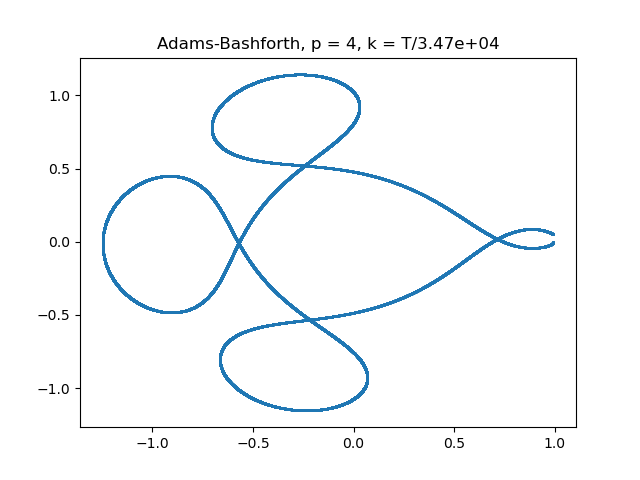
\includegraphics[scale = 0.45]{./report_src/Figure_8.png}
\end{figure}
因此我们得到,算法最大可行步长约为$n_{\max} = 3.47 \times 10^4$,略小于$p=3$时的最大可行步长。

\subsubsection{Adams-Moulton methods}
我们根据\textbf{Definition 11.83}和\textbf{Definition 11.84}编写了Adams-Moulton算法,需要注意的是我们需要用合适的方法获得足够的初始值进行迭代,因此,为了保证初始值的精度,我们采用五阶RK(因为$p$最大是5)获得足够的初始值。此外,关于每一步的迭代,由于迭代方程无法直接求解,因此我们采用不动点迭代进行每一步的求解。(对于轨道二也是如此,因此在2.3节中不再赘述)

$\bullet \;$ $p = 2$

首先,设置单周期数值求解步数$n = 2 \times 10^6$,绘制轨道一图像(作为直观展示)如下。此时轨道基本上没有肉眼可见的偏离,这是算法正确性的体现。
\begin{figure}[H]
\centering
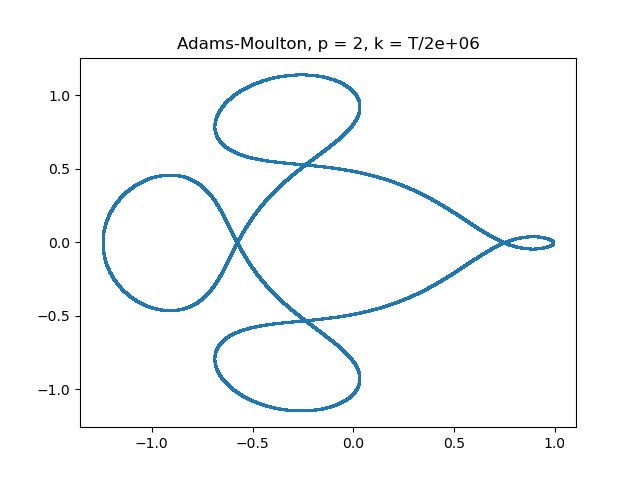
\includegraphics[scale = 0.45]{./report_src/Figure_9.png}
\end{figure}
其次,设置单周期数值求解步数分别为$n = 5 \times 10^5,1 \times 10^6,2 \times 10^6, 4 \times 10^6$(为了能得到相对准确的收敛阶,我们选取相对较大的$n$),得到$u_1$至$u_6$分量和初始值的绝对误差、对应算法收敛阶以及CPU time如下表所示:

\begin{table}[H]
\renewcommand{\arraystretch}{1.5}
\begin{center}
\begin{tabular}{c|c@{\hspace{0.2cm}}c
|c@{\hspace{0.2cm}}c|c@{\hspace{0.2cm}}c|c@{\hspace{0.2cm}}c}
  \hline
  \multirow{2}{*}{$\backslash$ \textbf{n}} & \multicolumn{2}{c|}{$5 \times 10^5$} & \multicolumn{2}{c|}{$1 \times 10^6$} & \multicolumn{2}{c|}{$2 \times 10^6$} & \multicolumn{2}{c}{$4 \times 10^6$} \\
  \cline{2-9}
  & 绝对误差&收敛阶 & 绝对误差 &收敛阶& 绝对误差 & 收敛阶 &绝对误差& 收敛阶 \\
  \hline
  $u_1$ & 2.321e-04 &$\backslash$  & 6.372e-05 &1.865 & 1.630e-05 &1.967 & 4.100e-06 &1.992 \\
$u_2$ & 9.059e-04 &$\backslash$  & 2.271e-04 &1.996 & 5.681e-05 &1.999 & 1.421e-05 &2.000 \\
$u_3$ & 0 &$\backslash$  & 0 &$\backslash$  & 0 &$\backslash$  & 0 &$\backslash$  \\
$u_4$ & 1.379e-01 &$\backslash$  & 3.632e-02 &1.924 & 9.192e-03 &1.982 & 2.305e-03 &1.996 \\
$u_5$ & 4.918e-02 &$\backslash$  & 1.080e-02 &2.187 & 2.594e-03 &2.058 & 6.416e-04 &2.015 \\
$u_6$ & 0 &$\backslash$  & 0 &$\backslash$  & 0 &$\backslash$  & 0 &$\backslash$  \\
\hline
平均收敛阶 & \multicolumn{2}{c|}{ $\backslash$ } & \multicolumn{2}{c|}{1.99} & \multicolumn{2}{c|}{2.00} & \multicolumn{2}{c}{2.00} \\
\hline
CPU time(ms) & \multicolumn{2}{c|}{520} & \multicolumn{2}{c|}{957} & \multicolumn{2}{c|}{1773} & \multicolumn{2}{c}{3389} \\
\hline

\end{tabular}
\end{center}
\end{table}
从中可以看出,随着$n$的增大,算法的收敛阶稳定在2,从而验证了算法的精度为2;CPU time与步数$n$基本成正比关系。另外,值得注意的是,和同阶的Adams-Bashforth算法相比,Adams-Moulton的误差似乎更小一些,但是由于不动点迭代求解的原因,所花费的时间也更多一些。

此外,以$10^2$为单位不断改变步数$n$,得到当$n = 5.93 \times 10^4$时,$u_1$和$u_2$的误差较大值为$4.95 \times 10^{-2}$,最接近给定阈值$5 \times 10^{-2}$,从而产生肉眼可见的偏离如下(对比上文中的较精确图像):
\begin{figure}[H]
\centering
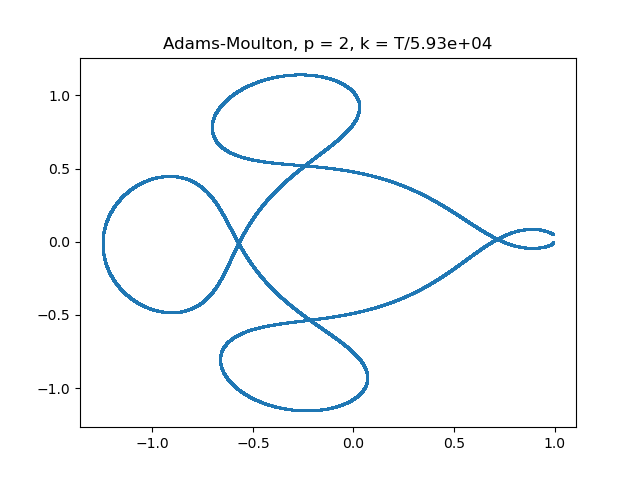
\includegraphics[scale = 0.45]{./report_src/Figure_10.png}
\end{figure}
因此我们得到,算法最大可行步长约为$n_{\max} = 5.93 \times 10^4$。

$\bullet \;$ $p = 3$

首先,设置单周期数值求解步数$n = 1 \times 10^5$,绘制轨道一图像(作为直观展示)如下。此时轨道基本上没有肉眼可见的偏离,这是算法正确性的体现。
\begin{figure}[H]
\centering
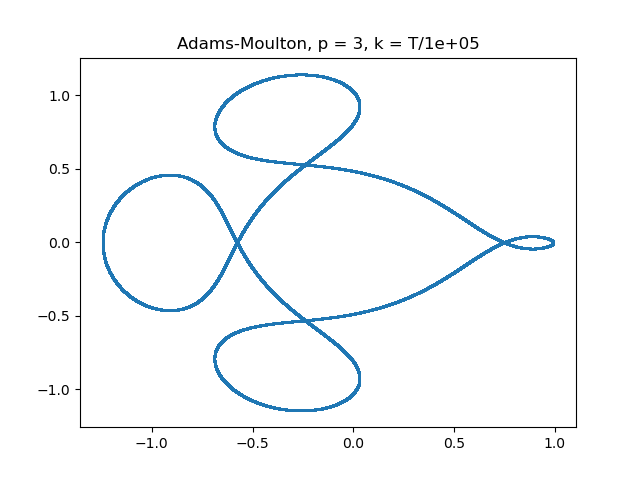
\includegraphics[scale = 0.45]{./report_src/Figure_11.png}
\end{figure}
其次,设置单周期数值求解步数分别为$n = 5 \times 10^5,1 \times 10^6,2 \times 10^6, 4 \times 10^6$(为了能得到相对准确的收敛阶,我们选取相对较大的$n$),得到$u_1$至$u_6$分量和初始值的绝对误差、对应算法收敛阶以及CPU time如下表所示:

\begin{table}[H]
\renewcommand{\arraystretch}{1.5}
\begin{center}
\begin{tabular}{c|c@{\hspace{0.2cm}}c
|c@{\hspace{0.2cm}}c|c@{\hspace{0.2cm}}c|c@{\hspace{0.2cm}}c}
  \hline
  \multirow{2}{*}{$\backslash$ \textbf{n}} & \multicolumn{2}{c|}{$5 \times 10^5$} & \multicolumn{2}{c|}{$1 \times 10^6$} & \multicolumn{2}{c|}{$2 \times 10^6$} & \multicolumn{2}{c}{$4 \times 10^6$} \\
  \cline{2-9}
  & 绝对误差&收敛阶 & 绝对误差 &收敛阶& 绝对误差 & 收敛阶 &绝对误差& 收敛阶 \\
  \hline
  $u_1$ & 7.565e-07 &$\backslash$  & 9.788e-08 &2.950 & 1.244e-08 &2.976 & 1.568e-09 &2.988 \\
$u_2$ & 2.674e-06 &$\backslash$  & 3.451e-07 &2.954 & 4.380e-08 &2.978 & 5.517e-09 &2.989 \\
$u_3$ & 0 &$\backslash$  & 0 &$\backslash$  & 0 &$\backslash$  & 0 &$\backslash$  \\
$u_4$ & 4.341e-04 &$\backslash$  & 5.602e-05 &2.954 & 7.112e-06 &2.978 & 8.958e-07 &2.989 \\
$u_5$ & 1.178e-04 &$\backslash$  & 1.523e-05 &2.952 & 1.935e-06 &2.976 & 2.439e-07 &2.988 \\
$u_6$ & 0 &$\backslash$  & 0 &$\backslash$  & 0 &$\backslash$  & 0 &$\backslash$  \\
\hline
平均收敛阶 & \multicolumn{2}{c|}{ $\backslash$ } & \multicolumn{2}{c|}{2.95} & \multicolumn{2}{c|}{2.98} & \multicolumn{2}{c}{2.99} \\
\hline
CPU time(ms) & \multicolumn{2}{c|}{613} & \multicolumn{2}{c|}{1204} & \multicolumn{2}{c|}{2296} & \multicolumn{2}{c}{4535} \\
\hline

\end{tabular}
\end{center}
\end{table}
从中可以看出,随着$n$的增大,算法的收敛阶稳定趋向于3,从而验证了算法的精度为3;CPU time与步数$n$基本成正比关系。另外,值得注意的是,和同阶的Adams-Bashforth算法相比,Adams-Moulton的误差似乎更小一些,但是由于不动点迭代求解的原因,所花费的时间也更多一些。

此外,以$10^2$为单位不断改变步数$n$,得到当$n = 1.31 \times 10^4$时,$u_1$和$u_2$的误差较大值为$4.95 \times 10^{-2}$,最接近给定阈值$5 \times 10^{-2}$,从而产生肉眼可见的偏离如下(对比上文中的较精确图像):
\begin{figure}[H]
\centering
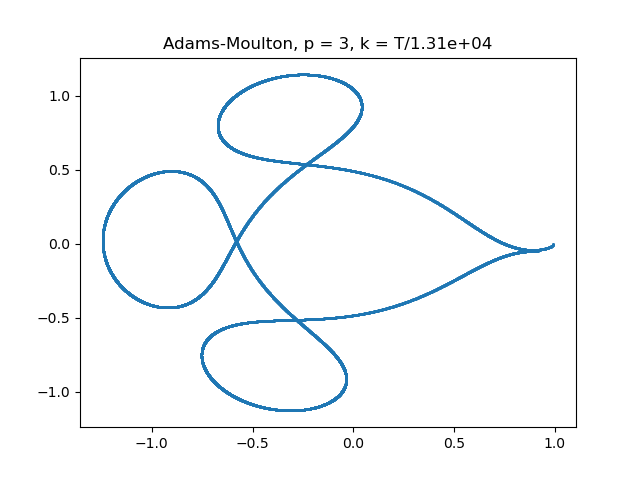
\includegraphics[scale = 0.45]{./report_src/Figure_12.png}
\end{figure}
因此我们得到,算法最大可行步长约为$n_{\max} = 1.31 \times 10^4$,小于$p=2$时的最大可行步长。

$\bullet \;$ $p = 4$

首先,设置单周期数值求解步数$n = 5 \times 10^4$,绘制轨道一图像(作为直观展示)如下。此时轨道基本上没有肉眼可见的偏离,这是算法正确性的体现。
\begin{figure}[H]
\centering
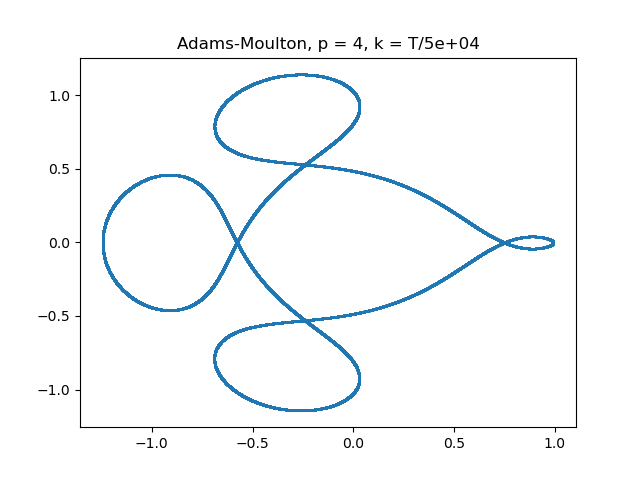
\includegraphics[scale = 0.45]{./report_src/Figure_13.png}
\end{figure}
其次,设置单周期数值求解步数分别为$n = 2 \times 10^5,4 \times 10^5,8 \times 10^5, 1.6 \times 10^6$(为了能得到相对准确的收敛阶,我们选取相对较大的$n$),得到$u_1$至$u_6$分量和初始值的绝对误差、对应算法收敛阶以及CPU time如下表所示:

\begin{table}[H]
\renewcommand{\arraystretch}{1.5}
\begin{center}
\begin{tabular}{c|c@{\hspace{0.2cm}}c
|c@{\hspace{0.2cm}}c|c@{\hspace{0.2cm}}c|c@{\hspace{0.2cm}}c}
  \hline
  \multirow{2}{*}{$\backslash$ \textbf{n}} & \multicolumn{2}{c|}{$2 \times 10^5$} & \multicolumn{2}{c|}{$4 \times 10^5$} & \multicolumn{2}{c|}{$8 \times 10^5$} & \multicolumn{2}{c}{$1.6 \times 10^6$} \\
  \cline{2-9}
  & 绝对误差&收敛阶 & 绝对误差 &收敛阶& 绝对误差 & 收敛阶 &绝对误差& 收敛阶 \\
  \hline
  $u_1$ & 2.335e-06 &$\backslash$  & 1.495e-07 &3.966 & 9.446e-09 &3.984 & 5.912e-10 &3.998 \\
$u_2$ & 7.850e-06 &$\backslash$  & 5.018e-07 &3.968 & 3.168e-08 &3.985 & 1.983e-09 &3.998 \\
$u_3$ & 0 &$\backslash$  & 0 &$\backslash$  & 0 &$\backslash$  & 0 &$\backslash$  \\
$u_4$ & 1.277e-03 &$\backslash$  & 8.157e-05 &3.968 & 5.150e-06 &3.985 & 3.224e-07 &3.998 \\
$u_5$ & 3.624e-04 &$\backslash$  & 2.326e-05 &3.962 & 1.470e-06 &3.984 & 9.202e-08 &3.998 \\
$u_6$ & 0 &$\backslash$  & 0 &$\backslash$  & 0 &$\backslash$  & 0 &$\backslash$  \\
\hline
平均收敛阶 & \multicolumn{2}{c|}{ $\backslash$ } & \multicolumn{2}{c|}{3.97} & \multicolumn{2}{c|}{3.98} & \multicolumn{2}{c}{4.00} \\
\hline
CPU time(ms) & \multicolumn{2}{c|}{404} & \multicolumn{2}{c|}{748} & \multicolumn{2}{c|}{1643} & \multicolumn{2}{c}{3302} \\
\hline

\end{tabular}
\end{center}
\end{table}
从中可以看出,随着$n$的增大,算法的收敛阶稳定趋向于4,从而验证了算法的精度为4;CPU time与步数$n$基本成正比关系。另外,值得注意的是,和同阶的Adams-Bashforth算法相比,Adams-Moulton的误差似乎更小一些,但是由于不动点迭代求解的原因,所花费的时间也更多一些。

此外,以$10^2$为单位不断改变步数$n$,得到当$n = 1.07 \times 10^4$时,$u_1$和$u_2$的误差较大值为$4.91 \times 10^{-2}$,最接近给定阈值$5 \times 10^{-2}$,从而产生肉眼可见的偏离如下(对比上文中的较精确图像):
\begin{figure}[H]
\centering
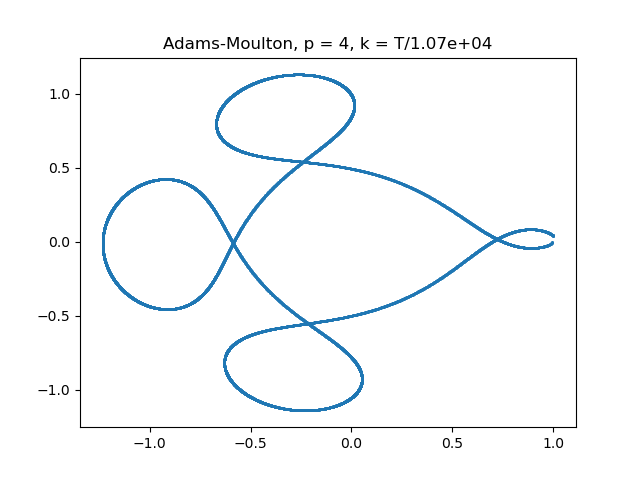
\includegraphics[scale = 0.45]{./report_src/Figure_14.png}
\end{figure}
因此我们得到,算法最大可行步长约为$n_{\max} = 1.07 \times 10^4$,小于$p=3$时的最大可行步长。

$\bullet \;$ $p = 5$

首先,设置单周期数值求解步数$n = 2.5 \times 10^4$,绘制轨道一图像(作为直观展示)如下。此时轨道基本上没有肉眼可见的偏离,这是算法正确性的体现。
\begin{figure}[H]
\centering
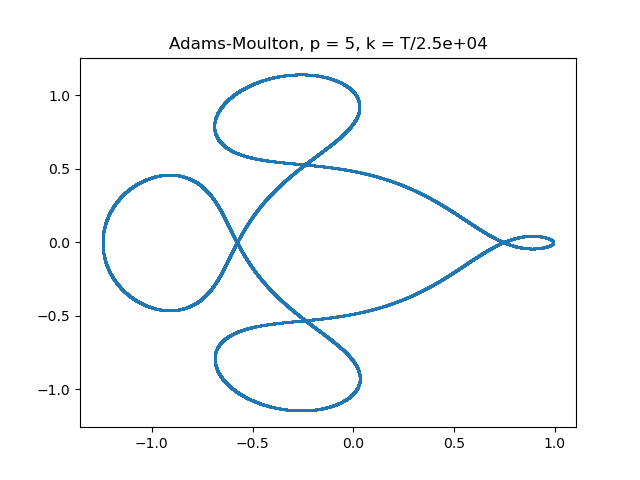
\includegraphics[scale = 0.45]{./report_src/Figure_15.png}
\end{figure}
其次,设置单周期数值求解步数分别为$n = 8 \times 10^4,1.6 \times 10^5,3.2 \times 10^5, 6.4 \times 10^5$(为了能得到相对准确的收敛阶,我们选取相对较大的$n$),得到$u_1$至$u_6$分量和初始值的绝对误差、对应算法收敛阶以及CPU time如下表所示:

\begin{table}[H]
\renewcommand{\arraystretch}{1.5}
\begin{center}
\begin{tabular}{c|c@{\hspace{0.2cm}}c
|c@{\hspace{0.2cm}}c|c@{\hspace{0.2cm}}c|c@{\hspace{0.2cm}}c}
  \hline
  \multirow{2}{*}{$\backslash$ \textbf{n}} & \multicolumn{2}{c|}{$8 \times 10^4$} & \multicolumn{2}{c|}{$1.6 \times 10^5$} & \multicolumn{2}{c|}{$3.2 \times 10^5$} & \multicolumn{2}{c}{$6.4 \times 10^5$} \\
  \cline{2-9}
  & 绝对误差&收敛阶 & 绝对误差 &收敛阶& 绝对误差 & 收敛阶 &绝对误差& 收敛阶 \\
  \hline
  $u_1$ & 5.171e-06 &$\backslash$  & 9.494e-08 &5.767 & 1.697e-09 &5.806 & 3.116e-11 &5.817 \\
$u_2$ & 1.654e-05 &$\backslash$  & 2.908e-07 &5.830 & 4.858e-09 &5.904 & 8.099e-11 &5.906 \\
$u_3$ & 0 &$\backslash$  & 0 &$\backslash$  & 0 &$\backslash$  & 0 &$\backslash$  \\
$u_4$ & 2.690e-03 &$\backslash$  & 4.739e-05 &5.827 & 7.933e-07 &5.901 & 1.327e-08 &5.902 \\
$u_5$ & 8.093e-04 &$\backslash$  & 1.478e-05 &5.775 & 2.641e-07 &5.806 & 4.853e-09 &5.816 \\
$u_6$ & 0 &$\backslash$  & 0 &$\backslash$  & 0 &$\backslash$  & 0 &$\backslash$  \\
\hline
平均收敛阶 & \multicolumn{2}{c|}{ $\backslash$ } & \multicolumn{2}{c|}{5.80} & \multicolumn{2}{c|}{5.84} & \multicolumn{2}{c}{5.85} \\
\hline
CPU time(ms) & \multicolumn{2}{c|}{204} & \multicolumn{2}{c|}{389} & \multicolumn{2}{c|}{749} & \multicolumn{2}{c}{1378} \\
\hline

\end{tabular}
\end{center}
\end{table}
从中可以看出,随着$n$的增大,算法的收敛阶趋向于5.85左右,我们在此进行如实汇报,但是正如您将在2.3节中所看到的,\textbf{对于轨道二该方法的收敛阶是准确的!关于其在轨道一的不稳定性的可能原因请见2.2.10节};CPU time与步数$n$基本成正比关系。

此外,以$10^1$为单位不断改变步数$n$,得到当$n = 8.89 \times 10^3$时,$u_1$和$u_2$的误差较大值为$4.92 \times 10^{-2}$,最接近给定阈值$5 \times 10^{-2}$,从而产生肉眼可见的偏离如下(对比上文中的较精确图像):
\begin{figure}[H]
\centering
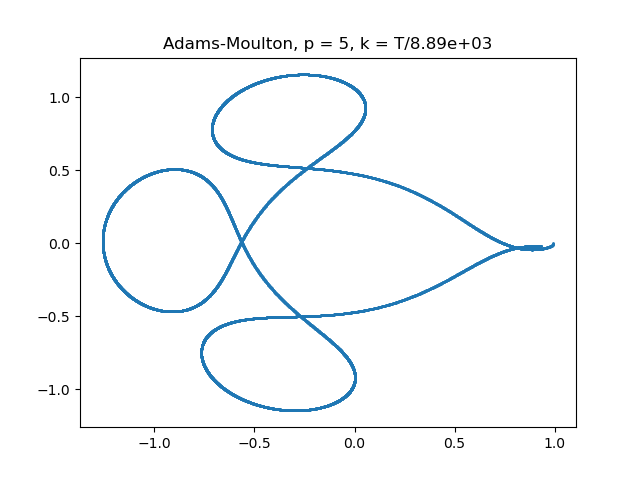
\includegraphics[scale = 0.45]{./report_src/Figure_16.png}
\end{figure}
因此我们得到,算法最大可行步长约为$n_{\max} = 8.89 \times 10^3$,小于$p=4$时的最大可行步长。

\subsubsection{BDFs}
我们根据\textbf{Definition 11.89}编写了BDF算法,需要注意的是我们需要用合适的方法获得足够的初始值进行迭代,因此,为了保证初始值的精度,我们采用经典四阶RK(因为$p$最大是4)获得足够的初始值。此外,关于每一步的迭代,由于迭代方程无法直接求解,因此我们采用不动点迭代进行每一步的求解。(对于轨道二也是如此,因此在2.3节中不再赘述)

$\bullet \;$ $p = 1$

首先,设置单周期数值求解步数$n = 2.5 \times 10^6$,绘制轨道一图像(作为直观展示)如下。此时轨道基本上没有肉眼可见的偏离,这是算法正确性的体现。
\begin{figure}[H]
\centering
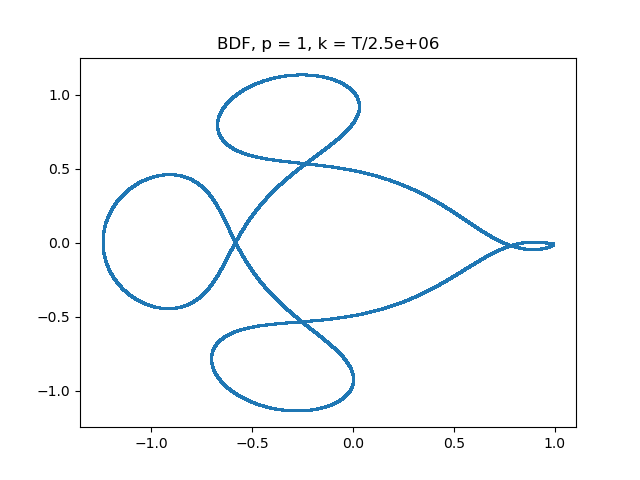
\includegraphics[scale = 0.45]{./report_src/Figure_17.png}
\end{figure}
其次,设置单周期数值求解步数分别为$n = 1 \times 10^7,2 \times 10^7,4 \times 10^7, 8 \times 10^7$($n$过大时不动点迭代会不收敛),得到$u_1$至$u_6$分量和初始值的绝对误差、对应算法收敛阶以及CPU time如下表所示:

\begin{table}[H]
\renewcommand{\arraystretch}{1.5}
\begin{center}
\begin{tabular}{c|c@{\hspace{0.2cm}}c
|c@{\hspace{0.2cm}}c|c@{\hspace{0.2cm}}c|c@{\hspace{0.2cm}}c}
  \hline
  \multirow{2}{*}{$\backslash$ \textbf{n}} & \multicolumn{2}{c|}{$1 \times 10^7$} & \multicolumn{2}{c|}{$2 \times 10^7$} & \multicolumn{2}{c|}{$4 \times 10^7$} & \multicolumn{2}{c}{$8 \times 10^7$} \\
  \cline{2-9}
  & 绝对误差&收敛阶 & 绝对误差 &收敛阶& 绝对误差 & 收敛阶 &绝对误差& 收敛阶 \\
  \hline
  $u_1$ & 9.532e-03 &$\backslash$  & 3.686e-03 &1.371 & 1.360e-03 &1.439 & 5.531e-04 &1.298 \\
$u_2$ & 8.512e-03 &$\backslash$  & 5.971e-03 &0.511 & 3.255e-03 &0.875 & 1.653e-03 &0.977 \\
$u_3$ & 0 &$\backslash$  & 0 &$\backslash$  & 0 &$\backslash$  & 0 &$\backslash$  \\
$u_4$ & 1.399e+00 &$\backslash$  & 1.095e+00 &0.353 & 6.037e-01 &0.859 & 2.922e-01 &1.047 \\
$u_5$ & 1.097e+00 &$\backslash$  & 3.694e-01 &1.570 & 2.856e-02 &3.693 & 3.065e-02 &-0.102 \\
$u_6$ & 0 &$\backslash$  & 0 &$\backslash$  & 0 &$\backslash$  & 0 &$\backslash$  \\
\hline
平均收敛阶 & \multicolumn{2}{c|}{ $\backslash$ } & \multicolumn{2}{c|}{0.95} & \multicolumn{2}{c|}{1.72} & \multicolumn{2}{c}{0.80} \\
\hline
CPU time(ms) & \multicolumn{2}{c|}{5938} & \multicolumn{2}{c|}{13233} & \multicolumn{2}{c|}{24449} & \multicolumn{2}{c}{43895} \\
\hline

\end{tabular}
\end{center}
\end{table}
从中可以看出,算法的收敛阶并不固定,我们在此进行如实汇报,但是正如您将在2.3节中所看到的,\textbf{对于轨道二该方法的收敛阶是准确的!关于其在轨道一的不稳定性的可能原因请见2.2.10节};CPU time与步数$n$基本成正比关系。

此外,以$10^4$为单位不断改变步数$n$,得到当$n = 1.25 \times 10^6$时,$u_1$和$u_2$的误差较大值为$4.96 \times 10^{-2}$,最接近给定阈值$5 \times 10^{-2}$,从而产生肉眼可见的偏离如下(对比上文中的较精确图像):
\begin{figure}[H]
\centering
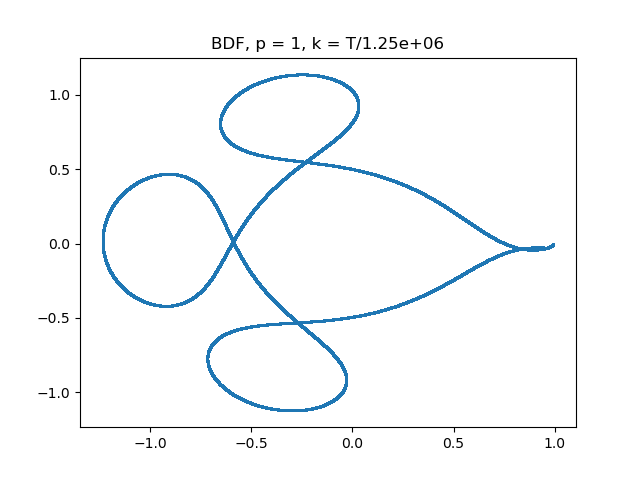
\includegraphics[scale = 0.45]{./report_src/Figure_18.png}
\end{figure}
因此我们得到,算法最大可行步长约为$n_{\max} = 1.25 \times 10^6$。

$\bullet \;$ $p = 2$

首先,设置单周期数值求解步数$n = 2 \times 10^6$,绘制轨道一图像(作为直观展示)如下。此时轨道基本上没有肉眼可见的偏离,这是算法正确性的体现。
\begin{figure}[H]
\centering
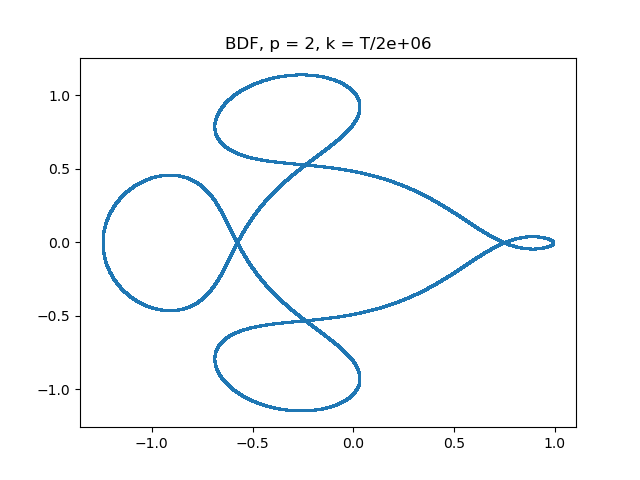
\includegraphics[scale = 0.45]{./report_src/Figure_19.png}
\end{figure}
其次,设置单周期数值求解步数分别为$n = 1 \times 10^6,2 \times 10^6,4 \times 10^6, 8 \times 10^6$(为了能得到相对准确的收敛阶,我们选取相对较大的$n$),得到$u_1$至$u_6$分量和初始值的绝对误差、对应算法收敛阶以及CPU time如下表所示:

\begin{table}[H]
\renewcommand{\arraystretch}{1.5}
\begin{center}
\begin{tabular}{c|c@{\hspace{0.2cm}}c
|c@{\hspace{0.2cm}}c|c@{\hspace{0.2cm}}c|c@{\hspace{0.2cm}}c}
  \hline
  \multirow{2}{*}{$\backslash$ \textbf{n}} & \multicolumn{2}{c|}{$1 \times 10^6$} & \multicolumn{2}{c|}{$2 \times 10^6$} & \multicolumn{2}{c|}{$4 \times 10^6$} & \multicolumn{2}{c}{$8 \times 10^6$} \\
  \cline{2-9}
  & 绝对误差&收敛阶 & 绝对误差 &收敛阶& 绝对误差 & 收敛阶 &绝对误差& 收敛阶 \\
  \hline
  $u_1$ & 2.308e-04 &$\backslash$  & 6.353e-05 &1.861 & 1.628e-05 &1.964 & 4.108e-06 &1.987 \\
$u_2$ & 9.007e-04 &$\backslash$  & 2.265e-04 &1.991 & 5.675e-05 &1.997 & 1.423e-05 &1.996 \\
$u_3$ & 0 &$\backslash$  & 0 &$\backslash$  & 0 &$\backslash$  & 0 &$\backslash$  \\
$u_4$ & 1.371e-01 &$\backslash$  & 3.622e-02 &1.921 & 9.182e-03 &1.980 & 2.309e-03 &1.992 \\
$u_5$ & 4.883e-02 &$\backslash$  & 1.076e-02 &2.182 & 2.590e-03 &2.055 & 6.429e-04 &2.011 \\
$u_6$ & 0 &$\backslash$  & 0 &$\backslash$  & 0 &$\backslash$  & 0 &$\backslash$  \\
\hline
平均收敛阶 & \multicolumn{2}{c|}{ $\backslash$ } & \multicolumn{2}{c|}{1.99} & \multicolumn{2}{c|}{2.00} & \multicolumn{2}{c}{2.00} \\
\hline
CPU time(ms) & \multicolumn{2}{c|}{831} & \multicolumn{2}{c|}{1413} & \multicolumn{2}{c|}{2625} & \multicolumn{2}{c}{4803} \\
\hline

\end{tabular}
\end{center}
\end{table}
从中可以看出,随着$n$的增大,算法的收敛阶稳定在2,从而验证了算法的精度为2;CPU time与步数$n$基本成正比关系。

此外,以$10^3$为单位不断改变步数$n$,得到当$n = 1.16 \times 10^5$时,$u_1$和$u_2$的误差较大值为$4.96 \times 10^{-2}$,最接近给定阈值$5 \times 10^{-2}$,从而产生肉眼可见的偏离如下(对比上文中的较精确图像):
\begin{figure}[H]
\centering
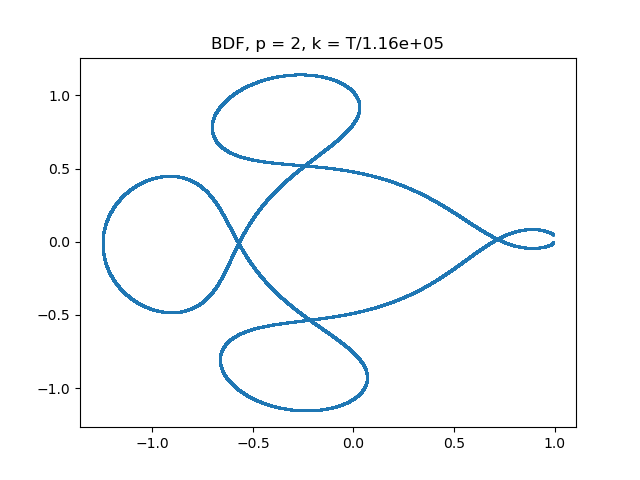
\includegraphics[scale = 0.45]{./report_src/Figure_20.png}
\end{figure}
因此我们得到,算法最大可行步长约为$n_{\max} = 1.16 \times 10^5$,远小于$p=1$时的最大可行步长。

$\bullet \;$ $p = 3$

首先,设置单周期数值求解步数$n = 1 \times 10^5$,绘制轨道一图像(作为直观展示)如下。此时轨道基本上没有肉眼可见的偏离,这是算法正确性的体现。
\begin{figure}[H]
\centering
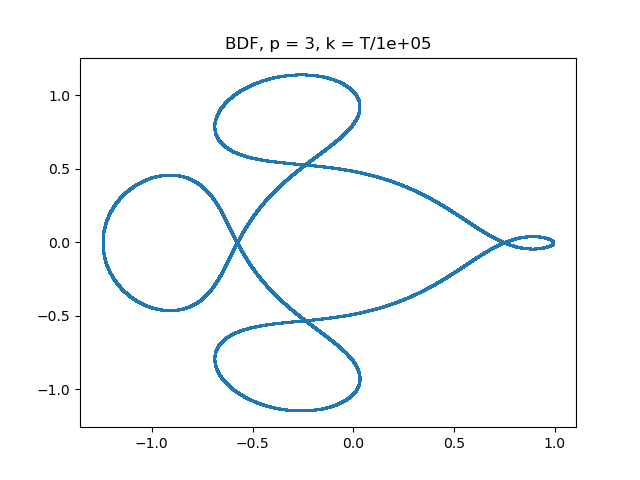
\includegraphics[scale = 0.45]{./report_src/Figure_21.png}
\end{figure}
其次,设置单周期数值求解步数分别为$n = 2.5 \times 10^5,5 \times 10^5,1 \times 10^6, 2 \times 10^6$(为了能得到相对准确的收敛阶,我们选取相对较大的$n$),得到$u_1$至$u_6$分量和初始值的绝对误差、对应算法收敛阶以及CPU time如下表所示:

\begin{table}[H]
\renewcommand{\arraystretch}{1.5}
\begin{center}
\begin{tabular}{c|c@{\hspace{0.2cm}}c
|c@{\hspace{0.2cm}}c|c@{\hspace{0.2cm}}c|c@{\hspace{0.2cm}}c}
  \hline
  \multirow{2}{*}{$\backslash$ \textbf{n}} & \multicolumn{2}{c|}{$2.5 \times 10^5$} & \multicolumn{2}{c|}{$5 \times 10^5$} & \multicolumn{2}{c|}{$1 \times 10^6$} & \multicolumn{2}{c}{$2 \times 10^6$} \\
  \cline{2-9}
  & 绝对误差&收敛阶 & 绝对误差 &收敛阶& 绝对误差 & 收敛阶 &绝对误差& 收敛阶 \\
  \hline
  $u_1$ & 4.261e-05 &$\backslash$  & 5.901e-06 &2.882 & 7.710e-07 &2.976 & 9.592e-08 &3.007 \\
$u_2$ & 1.706e-04 &$\backslash$  & 2.235e-05 &2.928 & 2.729e-06 &2.988 & 3.612e-07 &3.000 \\
$u_3$ & 0 &$\backslash$  & 0 &$\backslash$  & 0 &$\backslash$  & 0 &$\backslash$  \\
$u_4$ & 2.729e-02 &$\backslash$  & 3.499e-03 &2.916 & 4.430e-04 &2.987 & 5.539e-05 &3.000 \\
$u_5$ & 7.181e-03 &$\backslash$  & 9.138e-04 &2.950 & 1.200e-04 &2.987 & 1.492e-05 &3.008 \\
$u_6$ & 0 &$\backslash$  & 0 &$\backslash$  & 0 &$\backslash$  & 0 &$\backslash$  \\
\hline
平均收敛阶 & \multicolumn{2}{c|}{ $\backslash$ } & \multicolumn{2}{c|}{2.92} & \multicolumn{2}{c|}{2.98} & \multicolumn{2}{c}{3.00} \\
\hline
CPU time(ms) & \multicolumn{2}{c|}{263} & \multicolumn{2}{c|}{505} & \multicolumn{2}{c|}{1011} & \multicolumn{2}{c}{1935} \\
\hline
\end{tabular}
\end{center}
\end{table}
从中可以看出,随着$n$的增大,算法的收敛阶稳定趋向于3,从而验证了算法的精度为3;CPU time与步数$n$基本成正比关系。

此外,以$10^2$为单位不断改变步数$n$,得到当$n = 3.65 \times 10^4$时,$u_1$和$u_2$的误差较大值为$4.97 \times 10^{-2}$,最接近给定阈值$5 \times 10^{-2}$,从而产生肉眼可见的偏离如下(对比上文中的较精确图像):
\begin{figure}[H]
\centering
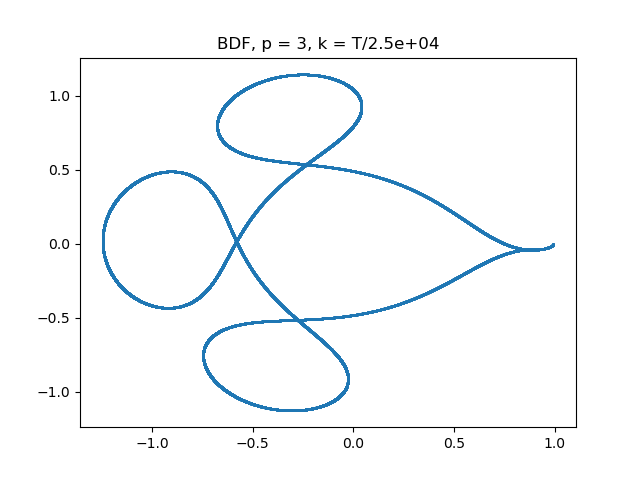
\includegraphics[scale = 0.45]{./report_src/Figure_22.png}
\end{figure}
因此我们得到,算法最大可行步长约为$n_{\max} = 3.65 \times 10^4$,远小于$p=2$时的最大可行步长。

$\bullet \;$ $p = 4$

首先,设置单周期数值求解步数$n = 8 \times 10^4$,绘制轨道一图像(作为直观展示)如下。此时轨道基本上没有肉眼可见的偏离,这是算法正确性的体现。
\begin{figure}[H]
\centering
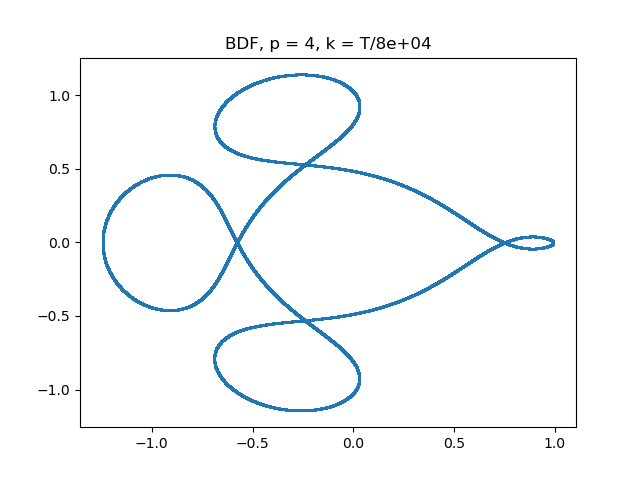
\includegraphics[scale = 0.45]{./report_src/Figure_23.png}
\end{figure}
其次,设置单周期数值求解步数分别为$n = 2 \times 10^5,4 \times 10^5,8 \times 10^5, 1.6 \times 10^6$(为了能得到相对准确的收敛阶,我们选取相对较大的$n$),得到$u_1$至$u_6$分量和初始值的绝对误差、对应算法收敛阶以及CPU time如下表所示:

\begin{table}[H]
\renewcommand{\arraystretch}{1.5}
\begin{center}
\begin{tabular}{c|c@{\hspace{0.2cm}}c
|c@{\hspace{0.2cm}}c|c@{\hspace{0.2cm}}c|c@{\hspace{0.2cm}}c}
  \hline
  \multirow{2}{*}{$\backslash$ \textbf{n}} & \multicolumn{2}{c|}{$2 \times 10^5$} & \multicolumn{2}{c|}{$4 \times 10^5$} & \multicolumn{2}{c|}{$8 \times 10^5$} & \multicolumn{2}{c}{$1.6 \times 10^6$} \\
  \cline{2-9}
  & 绝对误差&收敛阶 & 绝对误差 &收敛阶& 绝对误差 & 收敛阶 &绝对误差& 收敛阶 \\
  \hline
  $u_1$ & 1.718e-05 &$\backslash$  & 1.115e-06 &3.946 & 7.101e-08 &3.973 & 4.443e-09 &3.998 \\
$u_2$ & 5.754e-05 &$\backslash$  & 3.746e-06 &3.941 & 2.383e-07 &3.974 & 1.491e-08 &3.998 \\
$u_3$ & 0 &$\backslash$  & 0 &$\backslash$  & 0 &$\backslash$  & 0 &$\backslash$  \\
$u_4$ & 9.390e-03 &$\backslash$  & 6.091e-04 &3.946 & 3.874e-05 &3.975 & 2.424e-06 &3.998 \\
$u_5$ & 2.616e-03 &$\backslash$  & 1.733e-04 &3.917 & 1.105e-05 &3.971 & 6.915e-07 &3.998 \\
$u_6$ & 0 &$\backslash$  & 0 &$\backslash$  & 0 &$\backslash$  & 0 &$\backslash$  \\
\hline
平均收敛阶 & \multicolumn{2}{c|}{ $\backslash$ } & \multicolumn{2}{c|}{3.94} & \multicolumn{2}{c|}{3.97} & \multicolumn{2}{c}{4.00} \\
\hline
CPU time(ms) & \multicolumn{2}{c|}{272} & \multicolumn{2}{c|}{630} & \multicolumn{2}{c|}{939} & \multicolumn{2}{c}{1326} \\
\hline

\end{tabular}
\end{center}
\end{table}
从中可以看出,随着$n$的增大,算法的收敛阶稳定趋向于4,从而验证了算法的精度为4;CPU time与步数$n$基本成正比关系。

此外,以$10^2$为单位不断改变步数$n$,得到当$n = 3.25 \times 10^4$时,$u_1$和$u_2$的误差较大值为$4.91 \times 10^{-2}$,最接近给定阈值$5 \times 10^{-2}$,从而产生肉眼可见的偏离如下(对比上文中的较精确图像):
\begin{figure}[H]
\centering
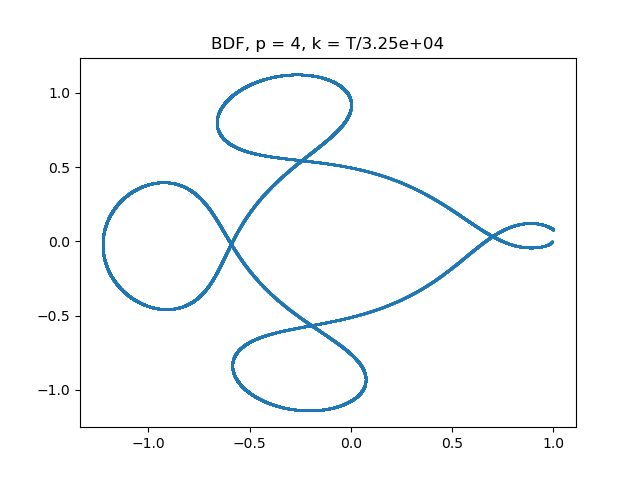
\includegraphics[scale = 0.45]{./report_src/Figure_24.png}
\end{figure}
因此我们得到,算法最大可行步长约为$n_{\max} = 3.25 \times 10^4$,略小于$p=3$时的最大可行步长。

\subsubsection{classical RK method}
我们根据\textbf{Definition 11.191}编写了classical RK算法,首先,设置单周期数值求解步数$n = 4 \times 10^4$(\textbf{关于项目作业要求的6000 steps的图像及其运行时间分析请见2.2.9节}),绘制轨道一图像(作为直观展示)如下。此时轨道基本上没有肉眼可见的偏离,这是算法正确性的体现。
\begin{figure}[H]
\centering
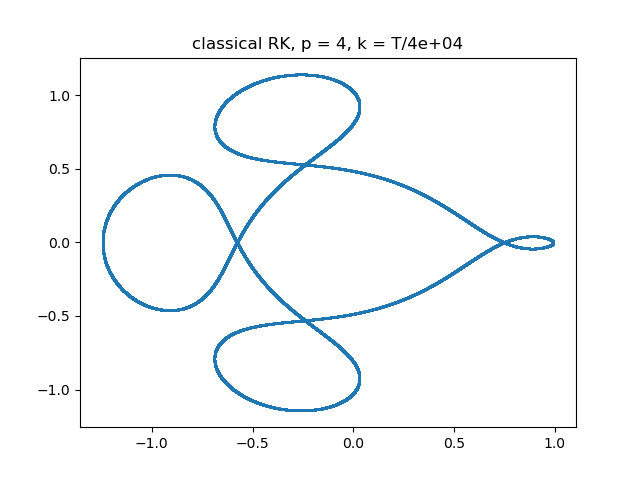
\includegraphics[scale = 0.45]{./report_src/Figure_25.png}
\end{figure}
其次,设置单周期数值求解步数分别为$n = 8 \times 10^4,1.6 \times 10^5,3.2 \times 10^5, 6.4 \times 10^5$(为了能得到相对准确的收敛阶,我们选取相对较大的$n$),得到$u_1$至$u_6$分量和初始值的绝对误差、对应算法收敛阶以及CPU time如下表所示:

\begin{table}[H]
\renewcommand{\arraystretch}{1.5}
\begin{center}
\begin{tabular}{c|c@{\hspace{0.2cm}}c
|c@{\hspace{0.2cm}}c|c@{\hspace{0.2cm}}c|c@{\hspace{0.2cm}}c}
  \hline
  \multirow{2}{*}{$\backslash$ \textbf{n}} & \multicolumn{2}{c|}{$8 \times 10^4$} & \multicolumn{2}{c|}{$1.6 \times 10^5$} & \multicolumn{2}{c|}{$3.2 \times 10^5$} & \multicolumn{2}{c}{$6.4 \times 10^5$} \\
  \cline{2-9}
  & 绝对误差&收敛阶 & 绝对误差 &收敛阶& 绝对误差 & 收敛阶 &绝对误差& 收敛阶 \\
  \hline
  $u_1$ & 2.576e-06 &$\backslash$  & 1.553e-07 &4.052 & 9.532e-09 &4.026 & 5.900e-10 &4.014 \\
$u_2$ & 8.099e-06 &$\backslash$  & 4.876e-07 &4.054 & 2.989e-08 &4.028 & 1.849e-09 &4.015 \\
$u_3$ & 0 &$\backslash$  & 0 &$\backslash$  & 0 &$\backslash$  & 0 &$\backslash$  \\
$u_4$ & 1.320e-03 &$\backslash$  & 7.943e-05 &4.055 & 4.870e-06 &4.028 & 3.012e-07 &4.015 \\
$u_5$ & 3.998e-04 &$\backslash$  & 2.417e-05 &4.048 & 1.484e-06 &4.026 & 9.183e-08 &4.014 \\
$u_6$ & 0 &$\backslash$  & 0 &$\backslash$  & 0 &$\backslash$  & 0 &$\backslash$  \\
\hline
平均收敛阶 & \multicolumn{2}{c|}{ $\backslash$ } & \multicolumn{2}{c|}{4.05} & \multicolumn{2}{c|}{4.03} & \multicolumn{2}{c}{4.01} \\
\hline
CPU time(ms) & \multicolumn{2}{c|}{67} & \multicolumn{2}{c|}{114} & \multicolumn{2}{c|}{217} & \multicolumn{2}{c}{409} \\
\hline

\end{tabular}
\end{center}
\end{table}
从中可以看出,随着$n$的增大,算法的收敛阶稳定趋向于4,从而验证了算法的精度为4;CPU time与步数$n$基本成正比关系。

此外,以$10^1$为单位不断改变步数$n$,得到当$n = 8.73 \times 10^3$时,$u_1$和$u_2$的误差较大值为$4.97 \times 10^{-2}$,最接近给定阈值$5 \times 10^{-2}$,从而产生肉眼可见的偏离如下(对比上文中的较精确图像):
\begin{figure}[H]
\centering
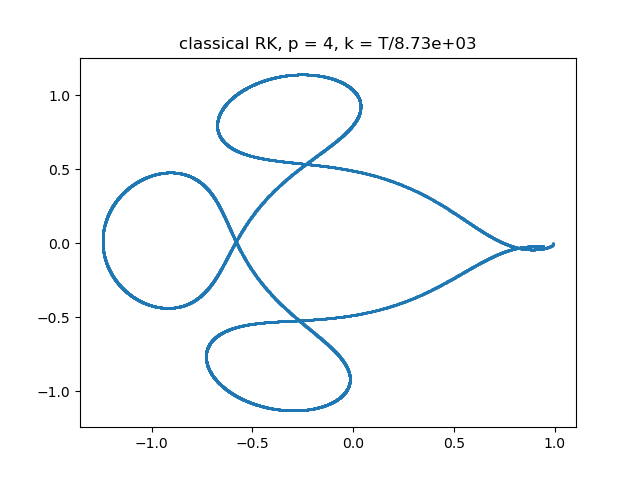
\includegraphics[scale = 0.45]{./report_src/Figure_26.png}
\end{figure}
因此我们得到,算法最大可行步长约为$n_{\max} = 8.73 \times 10^3$,相较之下小于Adams-Bashforth、Adams-Moulton以及BDF三种算法$p=4$时的最大可行步长。

\subsubsection{ESDIRK}
我们根据\textbf{Example 11.205}编写了ESDIRK算法,需要注意的是关于每一步的迭代,由于迭代方程无法直接求解,因此我们对每一步中每一个$\mathbf{y}_i$的求解都采用不动点迭代,并且带入$\mathbf{y}_{i+1}$的表达式中,从而得到每一轮迭代的结果。(对于轨道二也是如此,因此在2.3节中不再赘述)

首先,设置单周期数值求解步数$n = 4 \times 10^4$,绘制轨道一图像(作为直观展示)如下。此时轨道基本上没有肉眼可见的偏离,这是算法正确性的体现。
\begin{figure}[H]
\centering
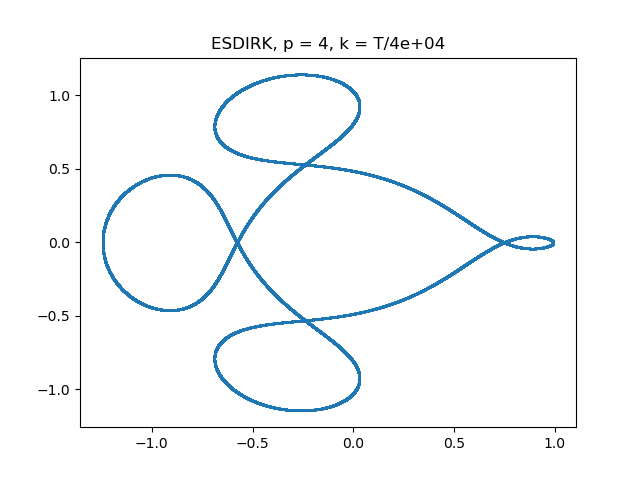
\includegraphics[scale = 0.45]{./report_src/Figure_27.png}
\end{figure}
其次,设置单周期数值求解步数分别为$n = 4 \times 10^4,8 \times 10^4,1.6 \times 10^5, 3.2 \times 10^5$(为了能得到相对准确的收敛阶,我们选取相对较大的$n$),得到$u_1$至$u_6$分量和初始值的绝对误差、对应算法收敛阶以及CPU time如下表所示:

\begin{table}[H]
\renewcommand{\arraystretch}{1.5}
\begin{center}
\begin{tabular}{c|c@{\hspace{0.2cm}}c
|c@{\hspace{0.2cm}}c|c@{\hspace{0.2cm}}c|c@{\hspace{0.2cm}}c}
  \hline
  \multirow{2}{*}{$\backslash$ \textbf{n}} & \multicolumn{2}{c|}{$4 \times 10^4$} & \multicolumn{2}{c|}{$8 \times 10^4$} & \multicolumn{2}{c|}{$1.6 \times 10^5$} & \multicolumn{2}{c}{$3.2 \times 10^5$} \\
  \cline{2-9}
  & 绝对误差&收敛阶 & 绝对误差 &收敛阶& 绝对误差 & 收敛阶 &绝对误差& 收敛阶 \\
  \hline
  $u_1$ & 1.414e-05 &$\backslash$  & 8.835e-07 &4.001 & 5.540e-08 &3.995 & 3.470e-09 &3.997 \\
$u_2$ & 4.574e-05 &$\backslash$  & 2.874e-06 &3.992 & 1.803e-07 &3.994 & 1.129e-08 &3.997 \\
$u_3$ & 0 &$\backslash$  & 0 &$\backslash$  & 0 &$\backslash$  & 0 &$\backslash$  \\
$u_4$ & 7.466e-03 &$\backslash$  & 4.677e-04 &3.997 & 2.934e-05 &3.995 & 1.838e-06 &3.997 \\
$u_5$ & 2.165e-03 &$\backslash$  & 1.374e-04 &3.978 & 8.623e-06 &3.994 & 5.401e-07 &3.997 \\
$u_6$ & 0 &$\backslash$  & 0 &$\backslash$  & 0 &$\backslash$  & 0 &$\backslash$  \\
\hline
平均收敛阶 & \multicolumn{2}{c|}{ $\backslash$ } & \multicolumn{2}{c|}{3.99} & \multicolumn{2}{c|}{3.99} & \multicolumn{2}{c}{4.00} \\
\hline
CPU time(ms) & \multicolumn{2}{c|}{260} & \multicolumn{2}{c|}{472} & \multicolumn{2}{c|}{742} & \multicolumn{2}{c}{1404} \\
\hline

\end{tabular}
\end{center}
\end{table}
从中可以看出,随着$n$的增大,算法的收敛阶稳定趋向于4,从而验证了算法的精度为4;CPU time与步数$n$近似成正比关系。值得注意的是,相较于classical RK method, ESDIRK在相同$n$的条件下拥有更小的误差和更稳定的收敛精度,不过由于需要进行不动点迭代,因此也牺牲了更多的运算时间。

此外,以$10^1$为单位不断改变步数$n$,得到当$n = 7.51 \times 10^3$时,$u_1$和$u_2$的误差较大值为$4.96 \times 10^{-2}$,最接近给定阈值$5 \times 10^{-2}$,从而产生肉眼可见的偏离如下(对比上文中的较精确图像):
\begin{figure}[H]
\centering
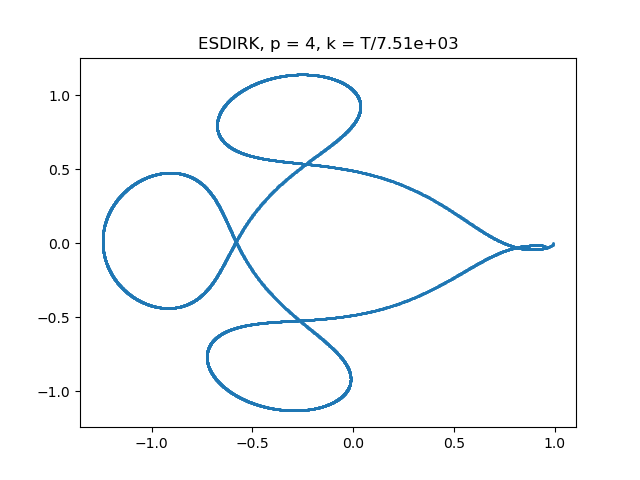
\includegraphics[scale = 0.45]{./report_src/Figure_28.png}
\end{figure}
因此我们得到,算法最大可行步长约为$n_{\max} = 7.51 \times 10^3$,相较之下小于Adams-Bashforth、Adams-Moulton、BDF,以及经典四阶RK四种算法$p=4$时的最大可行步长。

\subsubsection{Gauss-Legendre RK methods}
我们根据\textbf{Example 11.226}至\textbf{Example 11.228}编写了ESDIRK算法,需要注意的是关于每一步的迭代,由于迭代方程无法直接求解,因此我们对每一步中所有$\mathbf{y}_i$视为一个向量,作为整体进行不动点迭代(注意这与ESDIRK不同),从而得到每一轮迭代的结果。(对于轨道二也是如此,因此在2.3节中不再赘述)

$\bullet \;$ $p = 2(s=1)$

首先,设置单周期数值求解步数$n = 1 \times 10^6$,绘制轨道一图像(作为直观展示)如下。此时轨道基本上没有肉眼可见的偏离,这是算法正确性的体现。
\begin{figure}[H]
\centering
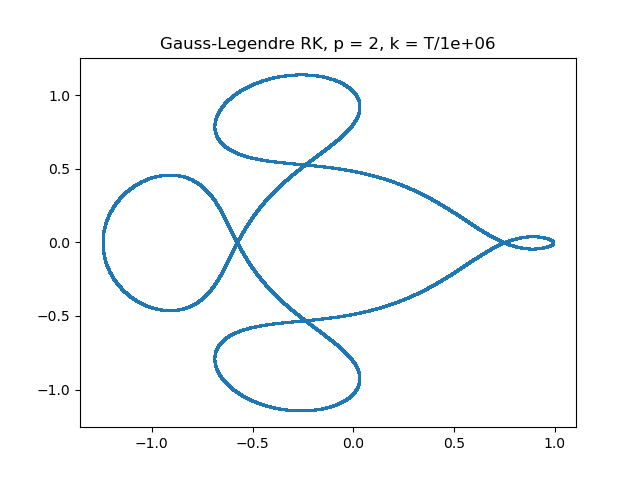
\includegraphics[scale = 0.45]{./report_src/Figure_29.png}
\end{figure}
其次,设置单周期数值求解步数分别为$n = 1 \times 10^6,2 \times 10^6,4 \times 10^6, 8 \times 10^6$(为了能得到相对准确的收敛阶,我们选取相对较大的$n$),得到$u_1$至$u_6$分量和初始值的绝对误差、对应算法收敛阶以及CPU time如下表所示:

\begin{table}[H]
\renewcommand{\arraystretch}{1.5}
\begin{center}
\begin{tabular}{c|c@{\hspace{0.2cm}}c
|c@{\hspace{0.2cm}}c|c@{\hspace{0.2cm}}c|c@{\hspace{0.2cm}}c}
  \hline
  \multirow{2}{*}{$\backslash$ \textbf{n}} & \multicolumn{2}{c|}{$1 \times 10^6$} & \multicolumn{2}{c|}{$2 \times 10^6$} & \multicolumn{2}{c|}{$4 \times 10^6$} & \multicolumn{2}{c}{$8 \times 10^6$} \\
  \cline{2-9}
  & 绝对误差&收敛阶 & 绝对误差 &收敛阶& 绝对误差 & 收敛阶 &绝对误差& 收敛阶 \\
  \hline
  $u_1$ & 7.758e-05 &$\backslash$  & 1.897e-05 &2.032 & 4.717e-06 &2.008 & 1.178e-06 &2.002 \\
$u_2$ & 2.388e-04 &$\backslash$  & 5.970e-05 &2.000 & 1.492e-05 &2.000 & 3.731e-06 &2.000 \\
$u_3$ & 0 &$\backslash$  & 0 &$\backslash$  & 0 &$\backslash$  & 0 &$\backslash$  \\
$u_4$ & 3.957e-02 &$\backslash$  & 9.764e-03 &2.019 & 2.433e-03 &2.005 & 6.078e-04 &2.001 \\
$u_5$ & 1.107e-02 &$\backslash$  & 2.892e-03 &1.937 & 7.304e-04 &1.985 & 1.831e-04 &1.996 \\
$u_6$ & 0 &$\backslash$  & 0 &$\backslash$  & 0 &$\backslash$  & 0 &$\backslash$  \\
\hline
平均收敛阶 & \multicolumn{2}{c|}{ $\backslash$ } & \multicolumn{2}{c|}{2.00} & \multicolumn{2}{c|}{2.00} & \multicolumn{2}{c}{2.00} \\
\hline
CPU time(ms) & \multicolumn{2}{c|}{1255} & \multicolumn{2}{c|}{2301} & \multicolumn{2}{c|}{4590} & \multicolumn{2}{c}{8892} \\
\hline

\end{tabular}
\end{center}
\end{table}
从中可以看出,随着$n$的增大,算法的收敛阶稳定在2,从而验证了算法的精度为2;CPU time与步数$n$近似成正比关系。此外,值得注意的是Gauss-Legendre RK方法2阶的误差要略小于Adams-Bashforth, Adams-Moulton, BDF对应的二阶算法误差,体现了算法的精确性。不过由于此时的不动点迭代是以向量为形式的,更为复杂,因此求解也更耗时。

此外,以$10^2$为单位不断改变步数$n$,得到当$n = 8.64 \times 10^4$时,$u_1$和$u_2$的误差较大值为$4.90 \times 10^{-2}$,最接近给定阈值$5 \times 10^{-2}$,从而产生肉眼可见的偏离如下(对比上文中的较精确图像):
\begin{figure}[H]
\centering
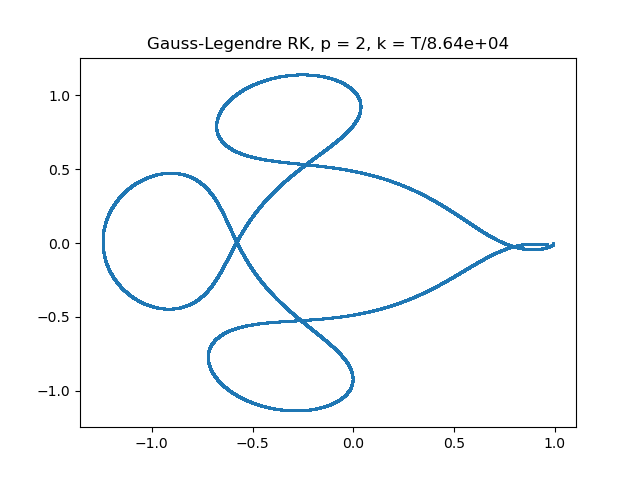
\includegraphics[scale = 0.45]{./report_src/Figure_30.png}
\end{figure}
因此我们得到,算法最大可行步长约为$n_{\max} = 8.64 \times 10^4$,小于Adams-Bashforth, Adams-Moulton, BDF对应的二阶算法的最大可行步长。

$\bullet \;$ $p = 4(s=2)$

首先,设置单周期数值求解步数$n = 4 \times 10^4$,绘制轨道一图像(作为直观展示)如下。此时轨道基本上没有肉眼可见的偏离,这是算法正确性的体现。
\begin{figure}[H]
\centering
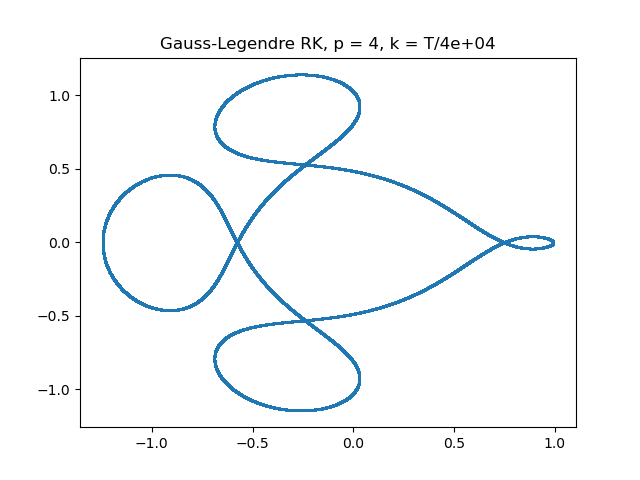
\includegraphics[scale = 0.45]{./report_src/Figure_31.png}
\end{figure}
其次,设置单周期数值求解步数分别为$n = 4 \times 10^4,8 \times 10^4,1.6 \times 10^5, 3.2 \times 10^5$(为了能得到相对准确的收敛阶,我们选取相对较大的$n$),得到$u_1$至$u_6$分量和初始值的绝对误差、对应算法收敛阶以及CPU time如下表所示:

\begin{table}[H]
\renewcommand{\arraystretch}{1.5}
\begin{center}
\begin{tabular}{c|c@{\hspace{0.2cm}}c
|c@{\hspace{0.2cm}}c|c@{\hspace{0.2cm}}c|c@{\hspace{0.2cm}}c}
  \hline
  \multirow{2}{*}{$\backslash$ \textbf{n}} & \multicolumn{2}{c|}{$4 \times 10^4$} & \multicolumn{2}{c|}{$8 \times 10^4$} & \multicolumn{2}{c|}{$1.6 \times 10^5$} & \multicolumn{2}{c}{$3.2 \times 10^5$} \\
  \cline{2-9}
  & 绝对误差&收敛阶 & 绝对误差 &收敛阶& 绝对误差 & 收敛阶 &绝对误差& 收敛阶 \\
  \hline
  $u_1$ & 1.032e-05 &$\backslash$  & 6.468e-07 &3.995 & 4.048e-08 &3.998 & 2.531e-09 &3.999 \\
$u_2$ & 3.023e-05 &$\backslash$  & 1.903e-06 &3.990 & 1.191e-07 &3.997 & 7.450e-09 &3.999 \\
$u_3$ & 0 &$\backslash$  & 0 &$\backslash$  & 0 &$\backslash$  & 0 &$\backslash$  \\
$u_4$ & 4.947e-03 &$\backslash$  & 3.107e-04 &3.993 & 1.945e-05 &3.998 & 1.216e-06 &3.999 \\
$u_5$ & 1.590e-03 &$\backslash$  & 1.006e-04 &3.982 & 6.301e-06 &3.997 & 3.940e-07 &3.999 \\
$u_6$ & 0 &$\backslash$  & 0 &$\backslash$  & 0 &$\backslash$  & 0 &$\backslash$  \\
\hline
平均收敛阶 & \multicolumn{2}{c|}{ $\backslash$ } & \multicolumn{2}{c|}{3.99} & \multicolumn{2}{c|}{4.00} & \multicolumn{2}{c}{4.00} \\
\hline
CPU time(ms) & \multicolumn{2}{c|}{126} & \multicolumn{2}{c|}{240} & \multicolumn{2}{c|}{453} & \multicolumn{2}{c}{864} \\
\hline

\end{tabular}
\end{center}
\end{table}
从中可以看出,随着$n$的增大,算法的收敛阶稳定在4,从而验证了算法的精度为4;CPU time与步数$n$近似成正比关系。此外,值得注意的是Gauss-Legendre RK方法4阶的误差要略小于Adams-Bashforth, Adams-Moulton, BDF对应的四阶算法误差,体现了算法的精确性。不过由于此时的不动点迭代是以向量为形式的,更为复杂,因此求解也更耗时。

此外,以$10^1$为单位不断改变步数$n$,得到当$n = 6.90 \times 10^3$时,$u_1$和$u_2$的误差较大值为$4.91 \times 10^{-2}$,最接近给定阈值$5 \times 10^{-2}$,从而产生肉眼可见的偏离如下(对比上文中的较精确图像):
\begin{figure}[H]
\centering
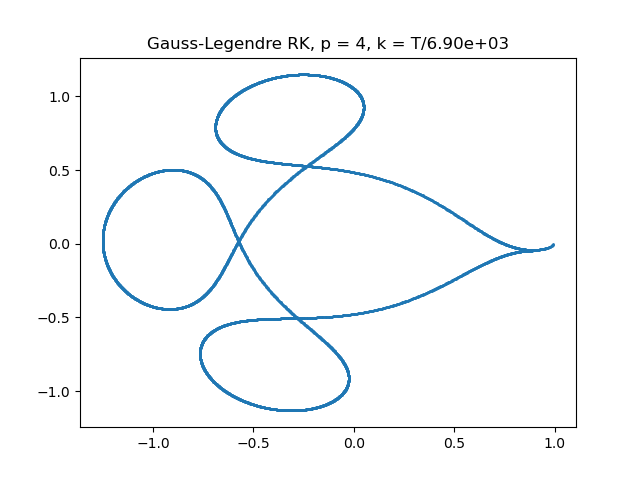
\includegraphics[scale = 0.45]{./report_src/Figure_32.png}
\end{figure}
因此我们得到,算法最大可行步长约为$n_{\max} = 6.90 \times 10^3$,小于Adams-Bashforth, Adams-Moulton, BDF对应的四阶算法的最大可行步长。

$\bullet \;$ $p = 6(s=3)$

首先,设置单周期数值求解步数$n = 1 \times 10^4$,绘制轨道一图像(作为直观展示)如下。此时轨道基本上没有肉眼可见的偏离,这是算法正确性的体现。
\begin{figure}[H]
\centering
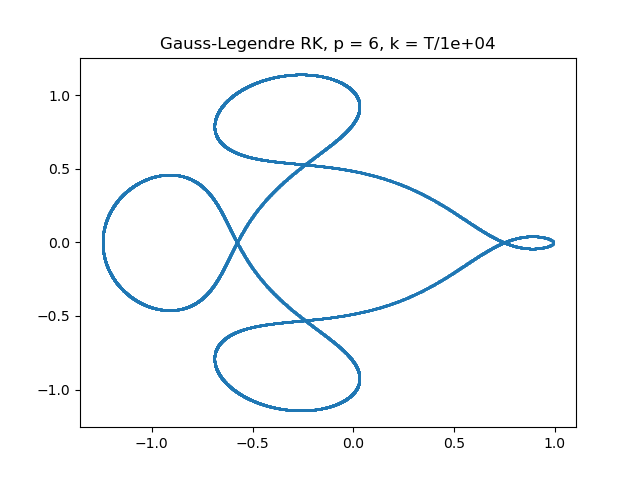
\includegraphics[scale = 0.45]{./report_src/Figure_33.png}
\end{figure}
其次,设置单周期数值求解步数分别为$n = 1 \times 10^4,2 \times 10^4,4 \times 10^5, 8 \times 10^4$(为了能得到相对准确的收敛阶,我们选取相对较大的$n$),得到$u_1$至$u_6$分量和初始值的绝对误差、对应算法收敛阶以及CPU time如下表所示:

\begin{table}[H]
\renewcommand{\arraystretch}{1.5}
\begin{center}
\begin{tabular}{c|c@{\hspace{0.2cm}}c
|c@{\hspace{0.2cm}}c|c@{\hspace{0.2cm}}c|c@{\hspace{0.2cm}}c}
  \hline
  \multirow{2}{*}{$\backslash$ \textbf{n}} & \multicolumn{2}{c|}{$1 \times 10^4$} & \multicolumn{2}{c|}{$2 \times 10^4$} & \multicolumn{2}{c|}{$4 \times 10^4$} & \multicolumn{2}{c}{$8 \times 10^4$} \\
  \cline{2-9}
  & 绝对误差&收敛阶 & 绝对误差 &收敛阶& 绝对误差 & 收敛阶 &绝对误差& 收敛阶 \\
  \hline
  $u_1$ & 5.418e-05 &$\backslash$  & 7.817e-07 &6.095 & 1.211e-08 &6.013 & 1.885e-10 &6.005 \\
$u_2$ & 1.679e-04 &$\backslash$  & 2.453e-06 &6.077 & 3.796e-08 &6.014 & 5.907e-10 &6.005 \\
$u_3$ & 0 &$\backslash$  & 0 &$\backslash$  & 0 &$\backslash$  & 0 &$\backslash$  \\
$u_4$ & 2.768e-02 &$\backslash$  & 3.997e-04 &6.094 & 6.183e-06 &6.014 & 9.624e-08 &6.005 \\
$u_5$ & 7.941e-03 &$\backslash$  & 1.216e-04 &6.019 & 1.884e-06 &6.012 & 2.934e-08 &6.004 \\
$u_6$ & 0 &$\backslash$  & 0 &$\backslash$  & 0 &$\backslash$  & 0 &$\backslash$  \\
\hline
平均收敛阶 & \multicolumn{2}{c|}{ $\backslash$ } & \multicolumn{2}{c|}{6.07} & \multicolumn{2}{c|}{6.01} & \multicolumn{2}{c}{6.00} \\
\hline
CPU time(ms) & \multicolumn{2}{c|}{60} & \multicolumn{2}{c|}{108} & \multicolumn{2}{c|}{210} & \multicolumn{2}{c}{393} \\
\hline

\end{tabular}
\end{center}
\end{table}
从中可以看出,随着$n$的增大,算法的收敛阶稳定在6,从而验证了算法的精度为6;CPU time与步数$n$近似成正比关系。

此外,以$10^1$为单位不断改变步数$n$,得到当$n = 2.77 \times 10^3$时,$u_1$和$u_2$的误差较大值为$4.96 \times 10^{-2}$,最接近给定阈值$5 \times 10^{-2}$,从而产生肉眼可见的偏离如下(对比上文中的较精确图像):
\begin{figure}[H]
\centering
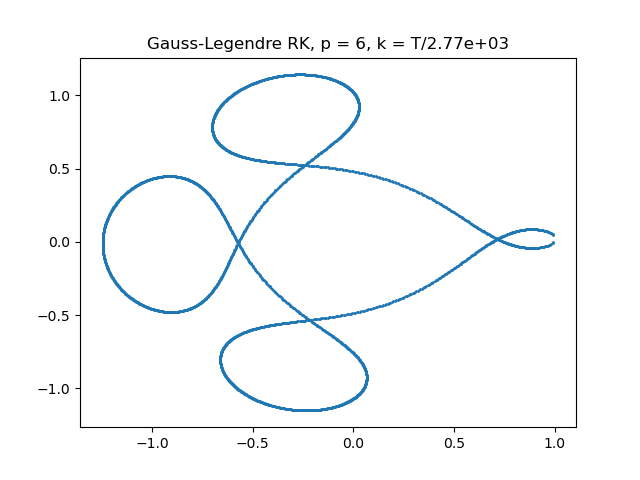
\includegraphics[scale = 0.45]{./report_src/Figure_34.png}
\end{figure}
因此我们得到,算法最大可行步长约为$n_{\max} = 2.77 \times 10^3$。

\subsubsection{Fehlberg 4(5) embedded RK method}
我们根据\textbf{Example 11.232}编写了Fehlberg 4(5) embedded RK method,首先,设置初始周期数值求解步长$\frac{T_1}{n}$,其中$n = 4 \times 10^4$,并取$\mathbf{E}_{abs}=\mathbf{E}_{rel}=10^{-8}$,$\rho_{max}=3.0$,$\rho = 0.8$,$\rho_{min} = 0.5$绘制轨道一图像(作为直观展示)如下。此时轨道基本上没有肉眼可见的偏离,这是算法正确性的体现。
\begin{figure}[H]
\centering
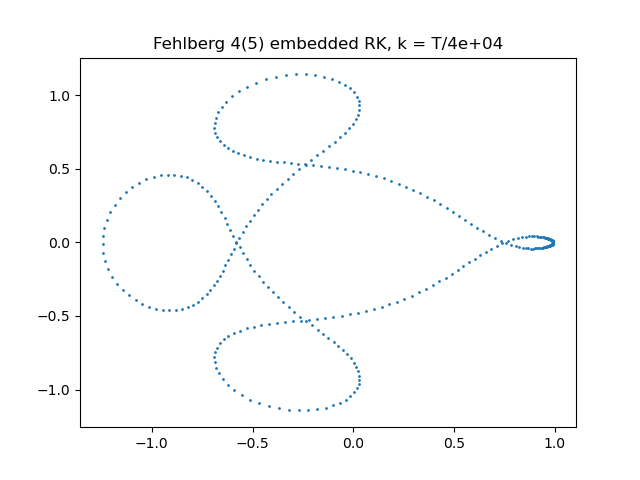
\includegraphics[scale = 0.45]{./report_src/Figure_35.png}
\end{figure}
其次,设置初始周期数值求解步长$\frac{T_1}{n}$,其中$n$分别为$n = 4 \times 10^4,8 \times 10^4,1.6 \times 10^5, 3.2 \times 10^5$,得到$u_1$至$u_6$分量和初始值的绝对误差、对应算法总步长、以及CPU time如下表所示(由于步长是自适应的,因此无法计算收敛阶):

\begin{table}[H]
\renewcommand{\arraystretch}{1.5}
\begin{center}
\begin{tabular}{c|c@{\hspace{0.2cm}}c
|c@{\hspace{0.2cm}}c|c@{\hspace{0.2cm}}c|c@{\hspace{0.2cm}}c}
  \hline
  \multirow{2}{*}{$\backslash$ \textbf{n(初始)}} & \multicolumn{2}{c|}{$4 \times 10^4$} & \multicolumn{2}{c|}{$8 \times 10^4$} & \multicolumn{2}{c|}{$1.6 \times 10^5$} & \multicolumn{2}{c}{$3.2 \times 10^5$} \\
  \cline{2-9}
  & 绝对误差&收敛阶 & 绝对误差 &收敛阶& 绝对误差 & 收敛阶 &绝对误差& 收敛阶 \\
  \hline
  $u_1$ & 2.893e-06 &$\backslash$  & 4.191e-06 &$\backslash$ & 9.338e-06 &$\backslash$ & 1.355e-05 &$\backslash$ \\
$u_2$ & 3.781e-05 &$\backslash$  & 1.865e-04 &$\backslash$ & 4.065e-04 &$\backslash$ & 5.247e-04 &$\backslash$ \\
$u_3$ & 0 &$\backslash$  & 0 &$\backslash$  & 0 &$\backslash$  & 0 &$\backslash$  \\
$u_4$ & 5.921e-02 &$\backslash$  & 2.937e-02 &$\backslash$ & 6.402e-03 &$\backslash$ & 8.258e-03 &$\backslash$ \\
$u_5$ & 4.241e-04 &$\backslash$  & 5.448e-04 &$\backslash$ & 1.621e-03 &$\backslash$ & 3.011e-04 &$\backslash$ \\
$u_6$ & 0 &$\backslash$  & 0 &$\backslash$  & 0 &$\backslash$  & 0 &$\backslash$  \\
\hline
对应算法总步长 & \multicolumn{2}{c|}{ 356} & \multicolumn{2}{c|}{356} & \multicolumn{2}{c|}{356} & \multicolumn{2}{c}{356} \\
\hline
CPU time(ms) & \multicolumn{2}{c|}{0.4} & \multicolumn{2}{c|}{0.4} & \multicolumn{2}{c|}{0.5} & \multicolumn{2}{c}{0.5} \\
\hline


\end{tabular}
\end{center}
\end{table}
从中可以看出,CPU time远小于之前的所有算法,并且不论初始的$n$是多少,对应算法总步长都是356,说明自适应算法能够很好的根据设定误差进行迭代。

\subsubsection{Dormand-Prince 5(4) embedded RK method}
我们根据\textbf{Example 11.233}编写了Dormand-Prince 5(4) embedded RK method,首先,设置初始周期数值求解步长$\frac{T_1}{n}$,其中$n = 2.5 \times 10^4$,并取$\mathbf{E}_{abs}=\mathbf{E}_{rel}=10^{-8}$,$\rho_{max}=3.0$,$\rho = 0.8$,$\rho_{min} = 0.5$绘制轨道一图像(作为直观展示)如下(\textbf{关于项目作业要求的100 steps的图像及其运行时间分析请见2.2.9节})。此时轨道基本上没有肉眼可见的偏离,这是算法正确性的体现。
\begin{figure}[H]
\centering
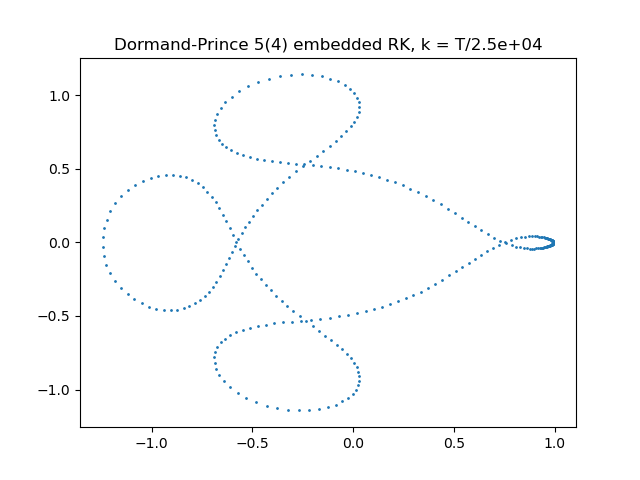
\includegraphics[scale = 0.45]{./report_src/Figure_36.png}
\end{figure}
其次,设置初始周期数值求解步长$\frac{T_1}{n}$,其中$n$分别为$n = 4 \times 10^4,8 \times 10^4,1.6 \times 10^5, 3.2 \times 10^5$,得到$u_1$至$u_6$分量和初始值的绝对误差、对应算法总步长、以及CPU time如下表所示(由于步长是自适应的,因此无法计算收敛阶):

\begin{table}[H]
\renewcommand{\arraystretch}{1.5}
\begin{center}
\begin{tabular}{c|c@{\hspace{0.2cm}}c
|c@{\hspace{0.2cm}}c|c@{\hspace{0.2cm}}c|c@{\hspace{0.2cm}}c}
  \hline
  \multirow{2}{*}{$\backslash$ \textbf{n(初始)}} & \multicolumn{2}{c|}{$4 \times 10^4$} & \multicolumn{2}{c|}{$8 \times 10^4$} & \multicolumn{2}{c|}{$1.6 \times 10^5$} & \multicolumn{2}{c}{$3.2 \times 10^5$} \\
  \cline{2-9}
  & 绝对误差&收敛阶 & 绝对误差 &收敛阶& 绝对误差 & 收敛阶 &绝对误差& 收敛阶 \\
  \hline
  $u_1$ & 5.767e-07 &$\backslash$  & 3.037e-06 &-2.397 & 9.494e-06 &-1.644 & 1.458e-05 &-0.619 \\
$u_2$ & 5.403e-05 &$\backslash$  & 2.558e-04 &-2.243 & 4.789e-04 &-0.905 & 5.988e-04 &-0.322 \\
$u_3$ & 0 &$\backslash$  & 0 &$\backslash$  & 0 &$\backslash$  & 0 &$\backslash$  \\
$u_4$ & 8.511e-03 &$\backslash$  & 4.030e-02 &-2.243 & 7.539e-02 &-0.904 & 9.418e-02 &-0.321 \\
$u_5$ & 3.549e-05 &$\backslash$  & 7.440e-04 &-4.390 & 2.786e-03 &-1.905 & 4.392e-03 &-0.657 \\
$u_6$ & 0 &$\backslash$  & 0 &$\backslash$  & 0 &$\backslash$  & 0 &$\backslash$  \\
\hline
对应算法总步长 & \multicolumn{2}{c|}{ 327} & \multicolumn{2}{c|}{327} & \multicolumn{2}{c|}{327} & \multicolumn{2}{c}{327} \\
\hline
CPU time(ms) & \multicolumn{2}{c|}{0.4} & \multicolumn{2}{c|}{0.4} & \multicolumn{2}{c|}{0.4} & \multicolumn{2}{c}{0.4} \\
\hline

\end{tabular}
\end{center}
\end{table}
从中可以看出,CPU time远小于非自适应步长的所有算法,并且不论初始的$n$是多少,对应算法总步长都是327说明自适应算法能够很好的根据设定误差进行迭代。

\subsubsection{其他:图像绘制及方法比较}
首先,分别绘制Euler's method with 24000 steps, classical RK methods with 6000 steps,和Dormand-Prince 5(4) embedded RK methods with 100 steps(经调整参数,当$\mathbf{E}_{abs}=\mathbf{E}_{rel}=2.3 \times 10^{-6}$,其他参数同上节不变时恰好一个周期走过100步)的图像如下所示。
\begin{figure}[H]
\centering
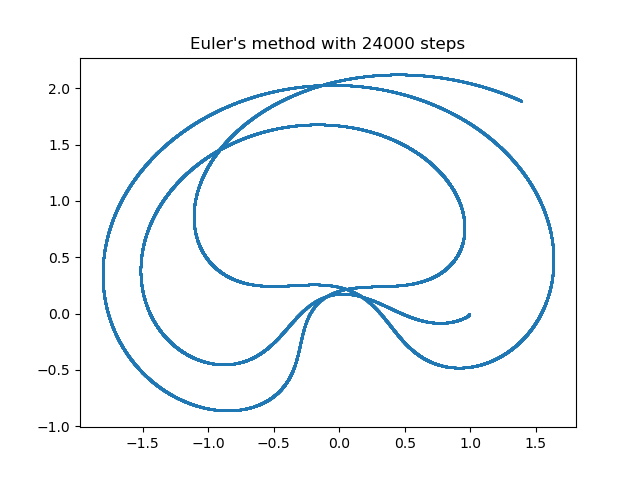
\includegraphics[scale = 0.45]{./report_src/Figure_37.png}
\end{figure}
\begin{figure}[H]
\centering
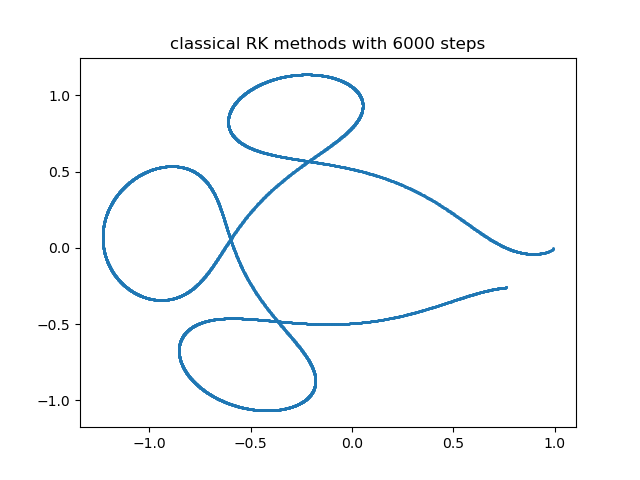
\includegraphics[scale = 0.45]{./report_src/Figure_38.png}
\end{figure}
\begin{figure}[H]
\centering
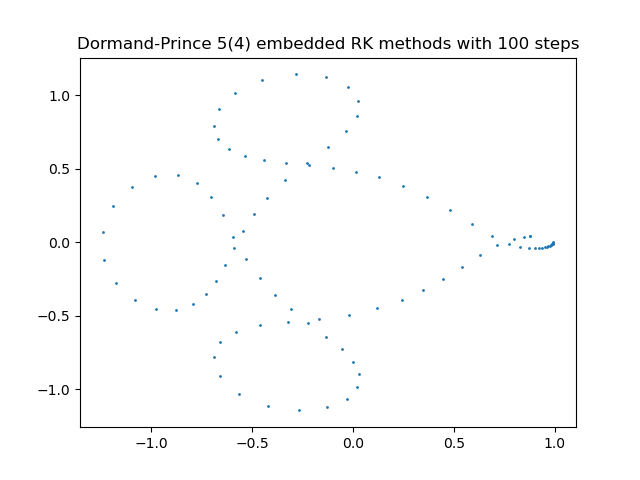
\includegraphics[scale = 0.45]{./report_src/Figure_39.png}
\end{figure}

显然,Euler's method with 24000 steps, classical RK methods with 6000 steps,和Dormand-Prince 5(4) embedded RK methods with 100 steps的图像依次变得更加精确。

此外,经过调整得到,为了达到$10^{-3}$的无穷范数误差:
\begin{itemize}
    \item 1.Euler's method 需要的步长大于$6 \times 10^7$, CPU time大于$15000$ms ;
    \item 2.classical RK method 需要的步长是$8.56 \times 10^4$, CPU time是$69$ms;
    \item 3.Dormand-Prince 5(4) embedded RK method 需要的步长是$5.19 \times 10^2$, CPU time是$0.5$ms;
\end{itemize}
很明显,Dormand-Prince 5(4) embedded RK method的CPU time最小。

\subsubsection{收敛阶误差简要分析}
鉴于在轨道一和轨道二经常会出现以下现象:某算法在其中一个轨道的收敛阶是精确的,而在另一个轨道的收敛阶是杂乱误差的。我们在此将其汇总如下:
\begin{itemize}
    \item 1.轨道一的所有一阶算法收敛阶都杂乱无章,但是轨道二的所有一阶算法都是准确的;
    \item 2.轨道一的AM五阶算法收敛阶杂乱无章,但是轨道二的对应算法都是准确的;
    \item 3.轨道二的除了GLRK的所有四阶算法收敛阶都杂乱无章,但是轨道一的所有四阶算法都是准确的。
\end{itemize}
我们可以发现出现问题的总是某一个阶数的大部分算法,因此可以首先确认这并不是程序设计有误,而是算法本身存在的问题。此外,由于其总是在某一个轨道正常而在另一个轨道的出现异常,因此我们可以断言是算法对于轨道的条件的不稳定造成的异常。

具体来说,我认为可能会有以下三个原因导致收敛阶出现异常:
\begin{itemize}
    \item 1.one-step error和周期误差并不是等价的。事实上,对于一个$p$阶精度的算法,前文已经得到one-step error为$\Theta(k^{p+1})$,而在运行一个周期之后的误差应是$\Theta(k^{p+1}) \times \frac{T}{k} = O(k^p)$的而不是$\Theta(k^{p})$。所以对其周期误差是单步误差的求和,可能会出现在$k$为步长时积累、在$\frac{k}{2}$为步长时抵消的情况(或者相反),因此通常来说并不能由此得到周期误差的收敛阶是$p$阶的。
    \item 2.不过,当$k$很小的时候,由于相邻两个点之间的导数变化较小(可近似视为相同),因此相邻两个one-step error会有更大的概率是同性质(都是累积或者都是抵消)的,我们由此可以得到此时的收敛阶应该是距离$p$阶较近的
    (这也是为什么我们总是选取较大的$n$测试收敛阶,哪怕较小的$n$已经误差足够小了)。然而,很小的$k$依旧会出现问题:误差太小,由于每一步的误差最小也得是机器精度,因此不可避免的造成收敛阶的测试异常,因为我们此时很难再得到更小的误差了。
    \item 3.此外,算法的条件数也会很大地影响收敛阶的稳定性。例如,我们发现Gauss-Legendre RK算法的四阶是稳定的,然而其余四阶算法对于轨道二都是不稳定的。并且隐式算法的稳定性要优于显示算法。这些都是因为算法的条件数不同,条件数越小的算法稳定性越高,从而可以得到更精确的收敛阶,或者说,收敛阶更加不受到函数和初始值的影响。

\end{itemize}

\subsection{轨道二结果展示}
根据项目要求,在这个部分,我对八个数值算法分别对八个轨道所有要求的精度$p$进行数值测试,并给出如下结果:
\begin{itemize}
    \item 1.\textbf{数值结果图像}。我将设置合适的单周期数值求解步数,绘制一幅$u_1$,$u_2$较为精确的图像作为直观展示;
    \item 2.\textbf{基于Richardson extrapolation的收敛阶计算}。这里Richardson外插的算法参考了LeVeque的课本附录A.6.3。具体来说,对于一个步长为$k$的数值算法其收敛阶计算方法如下:
\begin{itemize}
    \item 首先,计算步长为$k$,$\frac{k}{2}$,$\frac{k}{4}$时的计算解$\mathbf{U}(k)$,$\mathbf{U}(\frac{k}{2})$,$\mathbf{U}(\frac{k}{4})$;
    \item 其次,计算$\overline{\mathbf{E}}(k) = \mathbf{U}(k)-\mathbf{U}(\frac{k}{4})$,$\overline{\mathbf{E}}(\frac{k}{2}) = \mathbf{U}(\frac{k}{2})-\mathbf{U}(\frac{k}{4})$(不妨取绝对值);
    \item 第三,算法的收敛阶$p \approx \log_2 \left( \frac{\overline{\mathbf{E}}(k)}{\overline{\mathbf{E}}(\frac{k}{2})}-1 \right)$;
\end{itemize}
    \item 4.\textbf{算法CPU运行时间}。我将给出算法求解过程中的运行时间对比;
    \item 5.\textbf{算法最大可行步长 $n_{\max}$}。我将给出一个时间步长界,使得当步长再增大之后算法得到的图像就会产生肉眼可见的偏移。这里我们认为当$\overline{\mathbf{E}}(k)$中的$u_1$或者$u_2$分量达到$5 \times 10^{-2}$时,图像的偏移就会被肉眼观察到。
\end{itemize}
并且在本节的最后(2.2.9节),我将完成作业要求的最后部分,绘制并且比较Euler's method, classical RK method, Dormand-Prince 5(4) embedded RK method的相关图像和运行时间等。

\subsubsection{Adams-Bashforth methods}
$\bullet \;$ $p = 1$

首先,设置单周期数值求解步数$n = 8 \times 10^6$(\textbf{关于项目作业要求的24000 steps的图像及其运行时间分析请见2.3.9节}),绘制轨道一图像(作为直观展示)如下。此时轨道基本上没有肉眼可见的偏离,这是算法正确性的体现。
\begin{figure}[H]
\centering
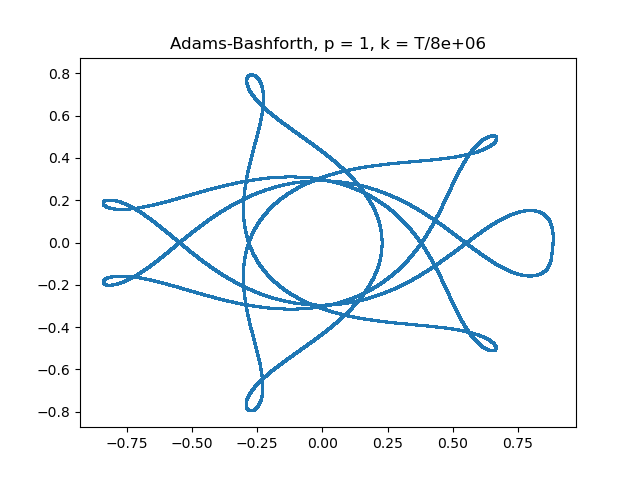
\includegraphics[scale = 0.45]{./report_src/Figure_40.png}
\end{figure}
其次,设置单周期数值求解步数分别为$n = 5 \times 10^6,1 \times 10^7, 2 \times 10^7$(为了能得到相对准确的收敛阶,我们选取相对较大的$n$),得到$u_1$至$u_6$分量和初始值的绝对误差、对应算法收敛阶以及CPU time如下表所示:

\begin{table}[H]
\renewcommand{\arraystretch}{1.5}
\begin{center}
\begin{tabular}{c|c@{\hspace{0.2cm}}c@{\hspace{0.2cm}}c
|c@{\hspace{0.2cm}}c@{\hspace{0.2cm}}c|c@{\hspace{0.2cm}}c@{\hspace{0.2cm}}c}
  \hline
  \multirow{2}{*}{$\backslash$ \textbf{n}} & \multicolumn{3}{c|}{$5 \times 10^6$} & \multicolumn{3}{c|}{$1 \times 10^7$} & \multicolumn{3}{c}{$2 \times 10^7$} \\
  \cline{2-10}
  &$\overline{\mathbf{E}}(k)$ & $\overline{\mathbf{E}}(\frac{k}{2})$&收敛阶 & $\overline{\mathbf{E}}(k)$ & $\overline{\mathbf{E}}(\frac{k}{2})$ &收敛阶& $\overline{\mathbf{E}}(k)$ & $\overline{\mathbf{E}}(\frac{k}{2})$ & 收敛阶  \\
  \hline
  $u_1$ & 8.162e-03 &2.649e-03 &1.057 & 3.949e-03 &1.300e-03 &1.027 & 1.943e-03 &6.438e-04 &1.013 \\
$u_2$ & 7.810e-03 &2.592e-03 &1.010 & 3.883e-03 &1.291e-03 &1.006 & 1.935e-03 &6.441e-04 &1.003 \\
$u_3$ & 0& 0 &$\backslash$  & 0& 0 &$\backslash$  & 0& 0 &$\backslash$  \\
$u_4$ & 3.722e-02 &1.174e-02 &1.118 & 1.738e-02 &5.641e-03 &1.057 & 8.406e-03 &2.766e-03 &1.028 \\
$u_5$ & 1.501e-02 &5.125e-03 &0.948 & 7.717e-03 &2.592e-03 &0.983 & 3.894e-03 &1.302e-03 &0.994 \\
$u_6$ & 0& 0 &$\backslash$  & 0& 0 &$\backslash$  & 0& 0 &$\backslash$  \\
\hline
平均收敛阶 & \multicolumn{3}{c|}{1.03} & \multicolumn{3}{c|}{1.02} & \multicolumn{3}{c}{1.01} \\
\hline
CPU time(ms) & \multicolumn{3}{c|}{1555} & \multicolumn{3}{c|}{3021} & \multicolumn{3}{c}{4048} \\
\hline

\end{tabular}
\end{center}
\end{table}
从中可以看出,随着$n$的增大,算法的收敛阶稳定在1,从而验证了算法的精度为1;CPU time与步数$n$基本成正比关系。

此外,以$10^4$为单位不断改变步数$n$,得到当$n = 1.15 \times 10^6$时,$u_1$和$u_2$的误差较大值为$4.98 \times 10^{-2}$,最接近给定阈值$5 \times 10^{-2}$,从而产生肉眼可见的偏离如下(对比上文中的较精确图像):
\begin{figure}[H]
\centering
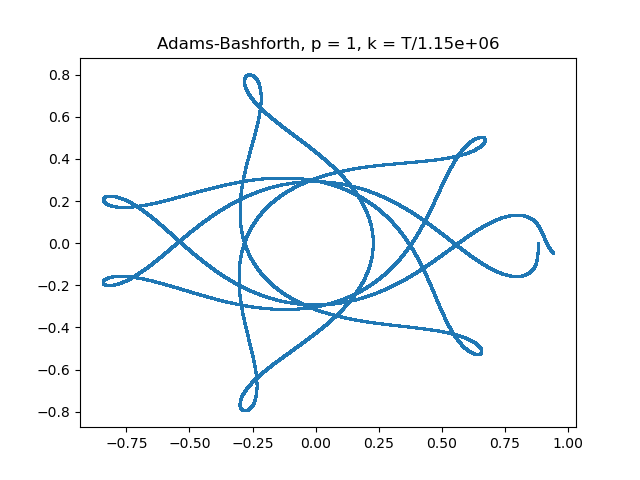
\includegraphics[scale = 0.45]{./report_src/Figure_41.png}
\end{figure}
因此我们得到,算法最大可行步长约为$n_{\max} = 1.15 \times 10^6$。

$\bullet \;$ $p = 2$

首先,设置单周期数值求解步数$n = 1 \times 10^6$,绘制轨道一图像(作为直观展示)如下。此时轨道基本上没有肉眼可见的偏离,这是算法正确性的体现。
\begin{figure}[H]
\centering
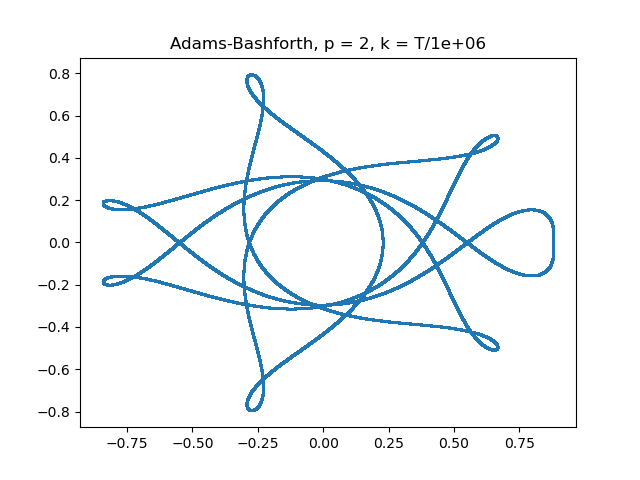
\includegraphics[scale = 0.45]{./report_src/Figure_42.png}
\end{figure}
其次,设置单周期数值求解步数分别为$n = 1 \times 10^6,2 \times 10^6,4 \times 10^6$(为了能得到相对准确的收敛阶,我们选取相对较大的$n$),得到$u_1$至$u_6$分量和初始值的绝对误差、对应算法收敛阶以及CPU time如下表所示:

\begin{table}[H]
\renewcommand{\arraystretch}{1.5}
\begin{center}
\begin{tabular}{c|c@{\hspace{0.2cm}}c@{\hspace{0.2cm}}c
|c@{\hspace{0.2cm}}c@{\hspace{0.2cm}}c|c@{\hspace{0.2cm}}c@{\hspace{0.2cm}}c}
  \hline
  \multirow{2}{*}{$\backslash$ \textbf{n}} & \multicolumn{3}{c|}{$1 \times 10^6$} & \multicolumn{3}{c|}{$2 \times 10^6$} & \multicolumn{3}{c}{$4 \times 10^6$} \\
  \cline{2-10}
  &$\overline{\mathbf{E}}(k)$ & $\overline{\mathbf{E}}(\frac{k}{2})$&收敛阶 & $\overline{\mathbf{E}}(k)$ & $\overline{\mathbf{E}}(\frac{k}{2})$ &收敛阶& $\overline{\mathbf{E}}(k)$ & $\overline{\mathbf{E}}(\frac{k}{2})$ & 收敛阶  \\
  \hline
  $u_1$ & 1.463e-07 &2.931e-08 &1.997 & 3.665e-08 &7.345e-09 &1.997 & 9.175e-09 &1.830e-09 &2.004 \\
$u_2$ & 4.243e-08 &8.430e-09 &2.012 & 1.052e-08 &2.090e-09 &2.012 & 2.618e-09 &5.281e-10 &1.985 \\
$u_3$ & 0& 0 &$\backslash$  & 0& 0 &$\backslash$  & 0& 0 &$\backslash$  \\
$u_4$ & 6.606e-07 &1.324e-07 &1.997 & 1.655e-07 &3.316e-08 &1.997 & 4.143e-08 &8.267e-09 &2.004 \\
$u_5$ & 2.666e-07 &5.342e-08 &1.996 & 6.681e-08 &1.339e-08 &1.996 & 1.673e-08 &3.336e-09 &2.005 \\
$u_6$ & 0& 0 &$\backslash$  & 0& 0 &$\backslash$  & 0& 0 &$\backslash$  \\
\hline
平均收敛阶 & \multicolumn{3}{c|}{2.00} & \multicolumn{3}{c|}{2.00} & \multicolumn{3}{c}{2.00} \\
\hline
CPU time(ms) & \multicolumn{3}{c|}{290} & \multicolumn{3}{c|}{577} & \multicolumn{3}{c}{1086} \\
\hline

\end{tabular}
\end{center}
\end{table}
从中可以看出,随着$n$的增大,算法的收敛阶稳定在2,从而验证了算法的精度为2;CPU time与步数$n$基本成正比关系。

此外,以$10^1$为单位不断改变步数$n$,得到当$n = 9.51 \times 10^3$时,$u_1$和$u_2$的误差较大值为$4.93 \times 10^{-2}$,最接近给定阈值$5 \times 10^{-2}$,从而产生肉眼可见的偏离如下(对比上文中的较精确图像):
\begin{figure}[H]
\centering
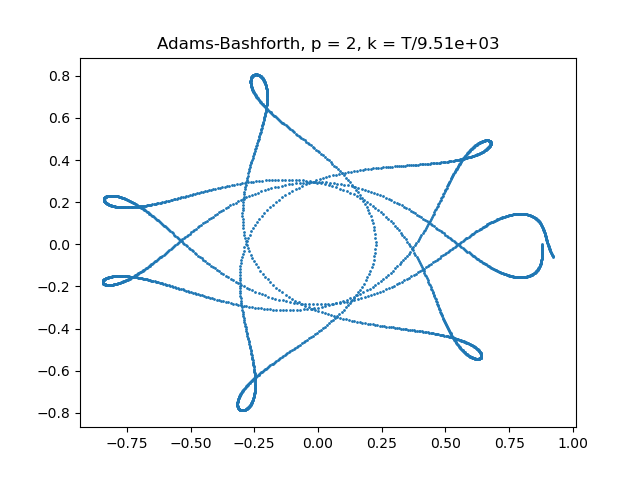
\includegraphics[scale = 0.45]{./report_src/Figure_43.png}
\end{figure}
因此我们得到,算法最大可行步长约为$n_{\max} = 9.51 \times 10^3$,远小于$p=1$时的最大可行步长。

$\bullet \;$ $p = 3$

首先,设置单周期数值求解步数$n = 1 \times 10^5$,绘制轨道一图像(作为直观展示)如下。此时轨道基本上没有肉眼可见的偏离,这是算法正确性的体现。
\begin{figure}[H]
\centering
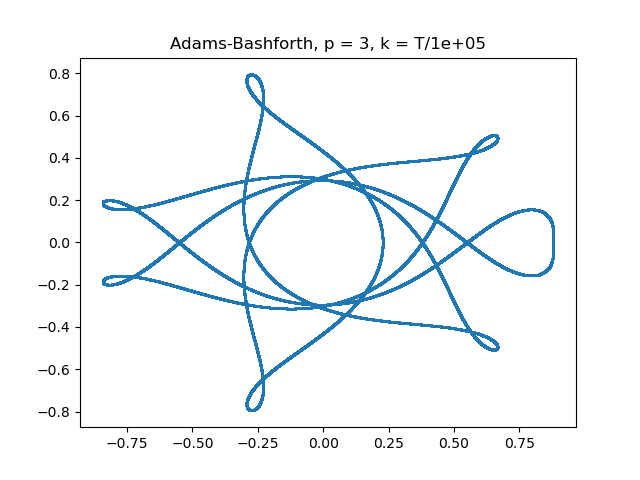
\includegraphics[scale = 0.45]{./report_src/Figure_44.png}
\end{figure}
其次,设置单周期数值求解步数分别为$n = 2 \times 10^4,4 \times 10^4,8 \times 10^4$(为了能得到相对准确的收敛阶,我们选取相对较大的$n$),得到$u_1$至$u_6$分量和初始值的绝对误差、对应算法收敛阶以及CPU time如下表所示:

\begin{table}[H]
\renewcommand{\arraystretch}{1.5}
\begin{center}
\begin{tabular}{c|c@{\hspace{0.2cm}}c@{\hspace{0.2cm}}c
|c@{\hspace{0.2cm}}c@{\hspace{0.2cm}}c|c@{\hspace{0.2cm}}c@{\hspace{0.2cm}}c}
  \hline
  \multirow{2}{*}{$\backslash$ \textbf{n}} & \multicolumn{3}{c|}{$2 \times 10^4$} & \multicolumn{3}{c|}{$4 \times 10^4$} & \multicolumn{3}{c}{$8 \times 10^4$} \\
  \cline{2-10}
  &$\overline{\mathbf{E}}(k)$ & $\overline{\mathbf{E}}(\frac{k}{2})$&收敛阶 & $\overline{\mathbf{E}}(k)$ & $\overline{\mathbf{E}}(\frac{k}{2})$ &收敛阶& $\overline{\mathbf{E}}(k)$ & $\overline{\mathbf{E}}(\frac{k}{2})$ & 收敛阶  \\
  \hline
  $u_1$ & 1.202e-04 &1.336e-05 &2.999 & 1.503e-05 &1.670e-06 &3.000 & 1.878e-06 &2.087e-07 &3.000 \\
$u_2$ & 1.209e-04 &1.344e-05 &3.000 & 1.512e-05 &1.680e-06 &3.000 & 1.890e-06 &2.100e-07 &3.000 \\
$u_3$ & 0& 0 &$\backslash$  & 0& 0 &$\backslash$  & 0& 0 &$\backslash$  \\
$u_4$ & 5.113e-04 &5.686e-05 &2.998 & 6.397e-05 &7.108e-06 &3.000 & 7.997e-06 &8.885e-07 &3.000 \\
$u_5$ & 2.455e-04 &2.727e-05 &3.000 & 3.068e-05 &3.409e-06 &3.000 & 3.835e-06 &4.261e-07 &3.000 \\
$u_6$ & 0& 0 &$\backslash$  & 0& 0 &$\backslash$  & 0& 0 &$\backslash$  \\
\hline
平均收敛阶 & \multicolumn{3}{c|}{3.00} & \multicolumn{3}{c|}{3.00} & \multicolumn{3}{c}{3.00} \\
\hline
CPU time(ms) & \multicolumn{3}{c|}{10} & \multicolumn{3}{c|}{18} & \multicolumn{3}{c}{38} \\
\hline

\end{tabular}
\end{center}
\end{table}
从中可以看出,随着$n$的增大,算法的收敛阶稳定于3,从而验证了算法的精度为3;CPU time与步数$n$基本成正比关系。

此外,以$10^1$为单位不断改变步数$n$,得到当$n = 3.53 \times 10^3$时,$u_1$和$u_2$的误差较大值为$4.90 \times 10^{-2}$,最接近给定阈值$5 \times 10^{-2}$,从而产生肉眼可见的偏离如下(对比上文中的较精确图像):
\begin{figure}[H]
\centering
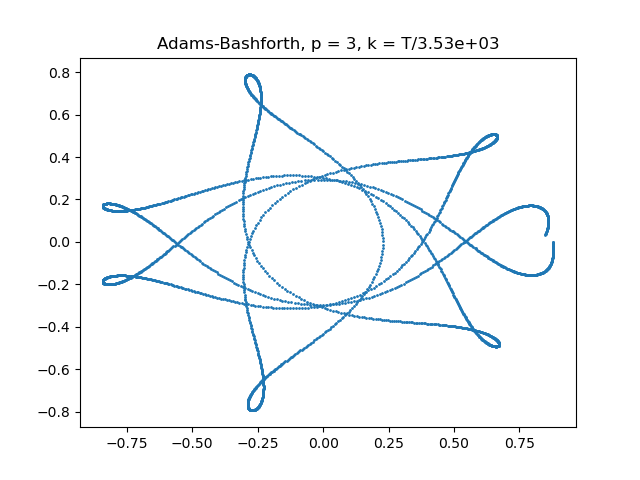
\includegraphics[scale = 0.45]{./report_src/Figure_45.png}
\end{figure}
因此我们得到,算法最大可行步长约为$n_{\max} = 3.53 \times 10^3$,远小于$p=2$时的最大可行步长。

$\bullet \;$ $p = 4$

首先,设置单周期数值求解步数$n = 2 \times 10^4$,绘制轨道一图像(作为直观展示)如下。此时轨道基本上没有肉眼可见的偏离,这是算法正确性的体现。
\begin{figure}[H]
\centering
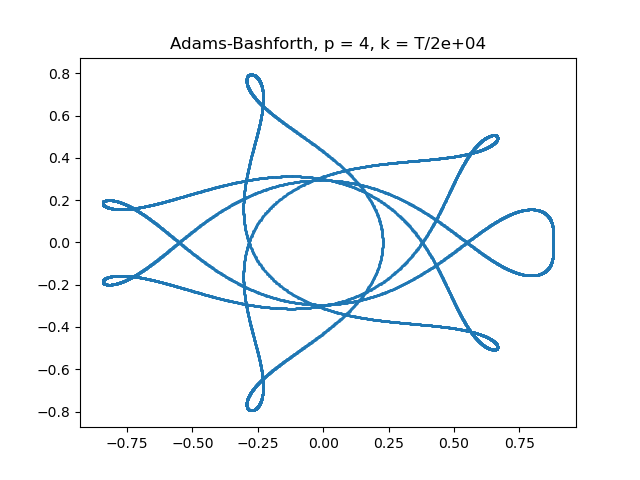
\includegraphics[scale = 0.45]{./report_src/Figure_46.png}
\end{figure}
其次,设置单周期数值求解步数分别为$n = 4 \times 10^4,8 \times 10^4,1.6 \times 10^5$(为了能得到相对准确的收敛阶,我们选取相对较大的$n$),得到$u_1$至$u_6$分量和初始值的绝对误差、对应算法收敛阶以及CPU time如下表所示:

\begin{table}[H]
\renewcommand{\arraystretch}{1.5}
\begin{center}
\begin{tabular}{c|c@{\hspace{0.2cm}}c@{\hspace{0.2cm}}c
|c@{\hspace{0.2cm}}c@{\hspace{0.2cm}}c|c@{\hspace{0.2cm}}c@{\hspace{0.2cm}}c}
  \hline
  \multirow{2}{*}{$\backslash$ \textbf{n}} & \multicolumn{3}{c|}{$4 \times 10^4$} & \multicolumn{3}{c|}{$8 \times 10^4$} & \multicolumn{3}{c}{$1.6 \times 10^5$} \\
  \cline{2-10}
  &$\overline{\mathbf{E}}(k)$ & $\overline{\mathbf{E}}(\frac{k}{2})$&收敛阶 & $\overline{\mathbf{E}}(k)$ & $\overline{\mathbf{E}}(\frac{k}{2})$ &收敛阶& $\overline{\mathbf{E}}(k)$ & $\overline{\mathbf{E}}(\frac{k}{2})$ & 收敛阶  \\
  \hline
  $u_1$ & 1.814e-09 &1.387e-10 &3.595 & 1.481e-10 &9.385e-12 &3.885 & 9.910e-12 &5.251e-13 &4.160 \\
$u_2$ & 1.805e-09 &7.412e-11 &4.545 & 7.800e-11 &3.879e-12 &4.256 & 4.166e-12 &2.866e-13 &3.759 \\
$u_3$ & 0& 0 &$\backslash$  & 0& 0 &$\backslash$  & 0& 0 &$\backslash$  \\
$u_4$ & 8.438e-09 &6.330e-10 &3.624 & 6.755e-10 &4.247e-11 &3.898 & 4.502e-11 &2.554e-12 &4.055 \\
$u_5$ & 3.081e-09 &2.460e-10 &3.527 & 2.630e-10 &1.703e-11 &3.853 & 1.783e-11 &8.034e-13 &4.406 \\
$u_6$ & 0& 0 &$\backslash$  & 0& 0 &$\backslash$  & 0& 0 &$\backslash$  \\
\hline
平均收敛阶 & \multicolumn{3}{c|}{3.82} & \multicolumn{3}{c|}{3.97} & \multicolumn{3}{c}{4.09} \\
\hline
CPU time(ms) & \multicolumn{3}{c|}{20} & \multicolumn{3}{c|}{37} & \multicolumn{3}{c}{88} \\
\hline

\end{tabular}
\end{center}
\end{table}
从中可以看出,随着$n$的增大,算法的收敛阶并没有稳定趋向于4(事实上改变$n$的值,收敛阶并不稳定),\textbf{然而该算法对于轨道一的收敛阶是精确的!关于收敛阶不稳定的可能原因,在2.2.10节中已经给出了相关分析};CPU time与步数$n$基本成正比关系。

此外,以$10^1$为单位不断改变步数$n$,得到当$n = 1.51 \times 10^3$时,$u_1$和$u_2$的误差较大值为$4.93 \times 10^{-2}$,最接近给定阈值$5 \times 10^{-2}$,从而产生肉眼可见的偏离如下(对比上文中的较精确图像):
\begin{figure}[H]
\centering
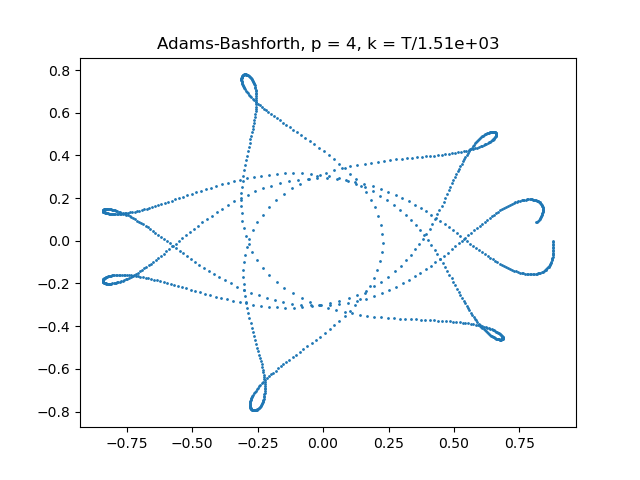
\includegraphics[scale = 0.45]{./report_src/Figure_47.png}
\end{figure}
因此我们得到,算法最大可行步长约为$n_{\max} = 1.51 \times 10^3$,小于$p=3$时的最大可行步长。

\subsubsection{Adams-Moulton methods}
$\bullet \;$ $p = 2$

首先,设置单周期数值求解步数$n = 1 \times 10^6$,绘制轨道一图像(作为直观展示)如下。此时轨道基本上没有肉眼可见的偏离,这是算法正确性的体现。
\begin{figure}[H]
\centering
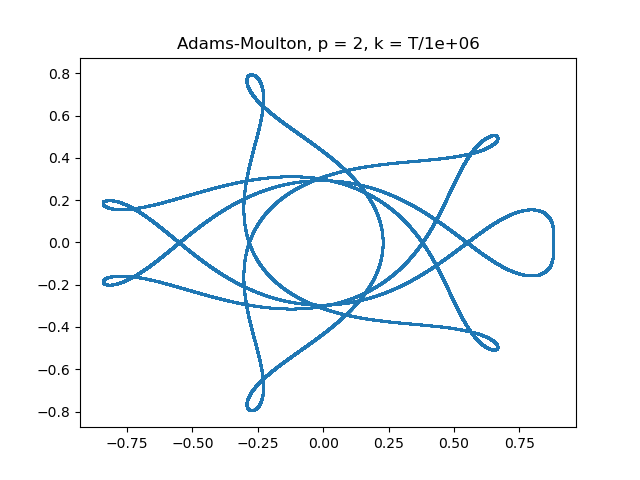
\includegraphics[scale = 0.45]{./report_src/Figure_48.png}
\end{figure}
其次,设置单周期数值求解步数分别为$n = 1 \times 10^5,2 \times 10^5, 4 \times 10^5$(为了能得到相对准确的收敛阶,我们选取相对较大的$n$),得到$u_1$至$u_6$分量和初始值的绝对误差、对应算法收敛阶以及CPU time如下表所示:

\begin{table}[H]
\renewcommand{\arraystretch}{1.5}
\begin{center}
\begin{tabular}{c|c@{\hspace{0.2cm}}c@{\hspace{0.2cm}}c
|c@{\hspace{0.2cm}}c@{\hspace{0.2cm}}c|c@{\hspace{0.2cm}}c@{\hspace{0.2cm}}c}
  \hline
  \multirow{2}{*}{$\backslash$ \textbf{n}} & \multicolumn{3}{c|}{$1 \times 10^5$} & \multicolumn{3}{c|}{$2 \times 10^5$} & \multicolumn{3}{c}{$4 \times 10^5$} \\
  \cline{2-10}
  &$\overline{\mathbf{E}}(k)$ & $\overline{\mathbf{E}}(\frac{k}{2})$&收敛阶 & $\overline{\mathbf{E}}(k)$ & $\overline{\mathbf{E}}(\frac{k}{2})$ &收敛阶& $\overline{\mathbf{E}}(k)$ & $\overline{\mathbf{E}}(\frac{k}{2})$ & 收敛阶  \\
  \hline
  $u_1$ & 2.938e-06 &5.876e-07 &2.000 & 7.346e-07 &1.469e-07 &2.000 & 1.836e-07 &3.673e-08 &2.000 \\
$u_2$ & 8.356e-07 &1.671e-07 &2.000 & 2.089e-07 &4.178e-08 &2.000 & 5.223e-08 &1.045e-08 &2.000 \\
$u_3$ & 0& 0 &$\backslash$  & 0& 0 &$\backslash$  & 0& 0 &$\backslash$  \\
$u_4$ & 1.327e-05 &2.653e-06 &2.000 & 3.317e-06 &6.633e-07 &2.000 & 8.292e-07 &1.658e-07 &2.000 \\
$u_5$ & 5.357e-06 &1.071e-06 &2.000 & 1.339e-06 &2.679e-07 &2.000 & 3.348e-07 &6.696e-08 &2.000 \\
$u_6$ & 0& 0 &$\backslash$  & 0& 0 &$\backslash$  & 0& 0 &$\backslash$  \\
\hline
平均收敛阶 & \multicolumn{3}{c|}{2.00} & \multicolumn{3}{c|}{2.00} & \multicolumn{3}{c}{2.00} \\
\hline
CPU time(ms) & \multicolumn{3}{c|}{133} & \multicolumn{3}{c|}{259} & \multicolumn{3}{c}{456} \\
\hline

\end{tabular}
\end{center}
\end{table}
从中可以看出,随着$n$的增大,算法的收敛阶稳定在2,从而验证了算法的精度为2;CPU time与步数$n$基本成正比关系。另外,值得注意的是,和同阶的Adams-Bashforth算法相比,Adams-Moulton的误差似乎更小一些,但是由于不动点迭代求解的原因,所花费的时间也更多一些。

此外,以$10^1$为单位不断改变步数$n$,得到当$n = 1.31 \times 10^3$时,$u_1$和$u_2$的误差较大值为$4.93 \times 10^{-2}$,最接近给定阈值$5 \times 10^{-2}$,从而产生肉眼可见的偏离如下(对比上文中的较精确图像):
\begin{figure}[H]
\centering
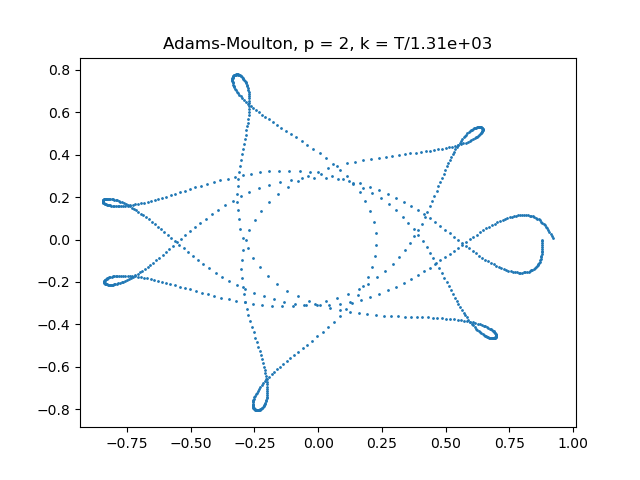
\includegraphics[scale = 0.45]{./report_src/Figure_49.png}
\end{figure}
因此我们得到,算法最大可行步长约为$n_{\max} = 1.31 \times 10^3$。

$\bullet \;$ $p = 3$

首先,设置单周期数值求解步数$n = 5 \times 10^4$,绘制轨道一图像(作为直观展示)如下。此时轨道基本上没有肉眼可见的偏离,这是算法正确性的体现。
\begin{figure}[H]
\centering
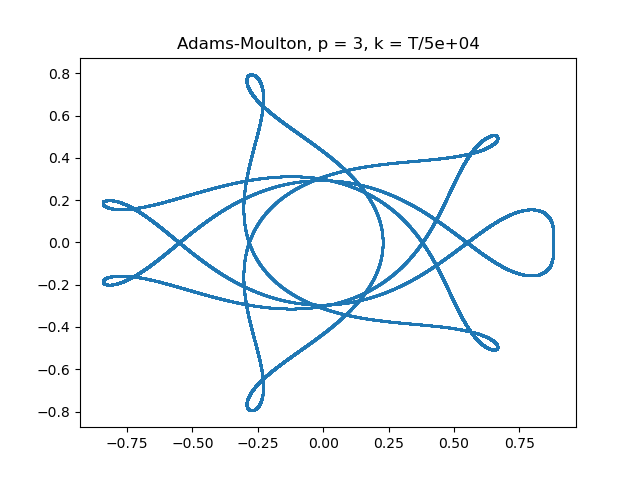
\includegraphics[scale = 0.45]{./report_src/Figure_50.png}
\end{figure}
其次,设置单周期数值求解步数分别为$n = 1 \times 10^4,2 \times 10^4,4 \times 10^4$(为了能得到相对准确的收敛阶,我们选取相对较大的$n$),得到$u_1$至$u_6$分量和初始值的绝对误差、对应算法收敛阶以及CPU time如下表所示:

\begin{table}[H]
\renewcommand{\arraystretch}{1.5}
\begin{center}
\begin{tabular}{c|c@{\hspace{0.2cm}}c@{\hspace{0.2cm}}c
|c@{\hspace{0.2cm}}c@{\hspace{0.2cm}}c|c@{\hspace{0.2cm}}c@{\hspace{0.2cm}}c}
  \hline
  \multirow{2}{*}{$\backslash$ \textbf{n}} & \multicolumn{3}{c|}{$1 \times 10^5$} & \multicolumn{3}{c|}{$2 \times 10^5$} & \multicolumn{3}{c}{$4 \times 10^5$} \\
  \cline{2-10}
  &$\overline{\mathbf{E}}(k)$ & $\overline{\mathbf{E}}(\frac{k}{2})$&收敛阶 & $\overline{\mathbf{E}}(k)$ & $\overline{\mathbf{E}}(\frac{k}{2})$ &收敛阶& $\overline{\mathbf{E}}(k)$ & $\overline{\mathbf{E}}(\frac{k}{2})$ & 收敛阶  \\
  \hline
 $u_1$ & 1.069e-04 &1.187e-05 &3.001 & 1.336e-05 &1.484e-06 &3.000 & 1.670e-06 &1.855e-07 &3.000 \\
$u_2$ & 1.075e-04 &1.194e-05 &3.000 & 1.344e-05 &1.493e-06 &3.000 & 1.680e-06 &1.866e-07 &3.000 \\
$u_3$ & 0& 0 &$\backslash$  & 0& 0 &$\backslash$  & 0& 0 &$\backslash$  \\
$u_4$ & 4.555e-04 &5.056e-05 &3.002 & 5.688e-05 &6.319e-06 &3.000 & 7.108e-06 &7.898e-07 &3.000 \\
$u_5$ & 2.181e-04 &2.424e-05 &3.000 & 2.727e-05 &3.030e-06 &3.000 & 3.408e-06 &3.787e-07 &3.000 \\
$u_6$ & 0& 0 &$\backslash$  & 0& 0 &$\backslash$  & 0& 0 &$\backslash$  \\
\hline
平均收敛阶 & \multicolumn{3}{c|}{3.00} & \multicolumn{3}{c|}{3.00} & \multicolumn{3}{c}{3.00} \\
\hline
CPU time(ms) & \multicolumn{3}{c|}{31} & \multicolumn{3}{c|}{48} & \multicolumn{3}{c}{93} \\
\hline

\end{tabular}
\end{center}
\end{table}
从中可以看出,随着$n$的增大,算法的收敛阶稳定趋向于3,从而验证了算法的精度为3;CPU time与步数$n$基本成正比关系。另外,值得注意的是,和同阶的Adams-Bashforth算法相比,Adams-Moulton的误差似乎更小一些,但是由于不动点迭代求解的原因,所花费的时间也更多一些。

此外,以$10^1$为单位不断改变步数$n$,得到当$n = 1.25 \times 10^3$时,$u_1$和$u_2$的误差较大值为$4.97 \times 10^{-2}$,最接近给定阈值$5 \times 10^{-2}$,从而产生肉眼可见的偏离如下(对比上文中的较精确图像):
\begin{figure}[H]
\centering
\includegraphics[scale = 0.45]{./report_src/Figure_51.png}
\end{figure}
因此我们得到,算法最大可行步长约为$n_{\max} = 1.25 \times 10^3$,略小于$p=2$时的最大可行步长。

$\bullet \;$ $p = 4$

首先,设置单周期数值求解步数$n = 2 \times 10^4$,绘制轨道一图像(作为直观展示)如下。此时轨道基本上没有肉眼可见的偏离,这是算法正确性的体现。
\begin{figure}[H]
\centering
\includegraphics[scale = 0.45]{./report_src/Figure_52.png}
\end{figure}
其次,设置单周期数值求解步数分别为$n = 1 \times 10^4,2 \times 10^4, 4 \times 10^4$(为了能得到相对准确的收敛阶,我们选取相对较大的$n$),得到$u_1$至$u_6$分量和初始值的绝对误差、对应算法收敛阶以及CPU time如下表所示:

\begin{table}[H]
\renewcommand{\arraystretch}{1.5}
\begin{center}
\begin{tabular}{c|c@{\hspace{0.2cm}}c@{\hspace{0.2cm}}c
|c@{\hspace{0.2cm}}c@{\hspace{0.2cm}}c|c@{\hspace{0.2cm}}c@{\hspace{0.2cm}}c}
  \hline
  \multirow{2}{*}{$\backslash$ \textbf{n}} & \multicolumn{3}{c|}{$1 \times 10^4$} & \multicolumn{3}{c|}{$2 \times 10^4$} & \multicolumn{3}{c}{$4 \times 10^4$} \\
  \cline{2-10}
  &$\overline{\mathbf{E}}(k)$ & $\overline{\mathbf{E}}(\frac{k}{2})$&收敛阶 & $\overline{\mathbf{E}}(k)$ & $\overline{\mathbf{E}}(\frac{k}{2})$ &收敛阶& $\overline{\mathbf{E}}(k)$ & $\overline{\mathbf{E}}(\frac{k}{2})$ & 收敛阶  \\
  \hline
 $u_1$ & 1.299e-08 &2.007e-09 &2.452 & 2.174e-09 &1.670e-10 &3.587 & 1.766e-10 &9.592e-12 &4.122 \\
$u_2$ & 5.720e-08 &2.118e-09 &4.701 & 2.209e-09 &9.080e-11 &4.544 & 9.724e-11 &6.443e-12 &3.817 \\
$u_3$ & 0& 0 &$\backslash$  & 0& 0 &$\backslash$  & 0& 0 &$\backslash$  \\
$u_4$ & 6.884e-08 &9.359e-09 &2.668 & 1.012e-08 &7.623e-10 &3.618 & 8.063e-10 &4.398e-11 &4.116 \\
$u_5$ & 1.474e-08 &3.389e-09 &1.744 & 3.685e-09 &2.960e-10 &3.517 & 3.129e-10 &1.689e-11 &4.132 \\
$u_6$ & 0& 0 &$\backslash$  & 0& 0 &$\backslash$  & 0& 0 &$\backslash$  \\
\hline
平均收敛阶 & \multicolumn{3}{c|}{2.89} & \multicolumn{3}{c|}{3.82} & \multicolumn{3}{c}{4.05} \\
\hline
CPU time(ms) & \multicolumn{3}{c|}{31} & \multicolumn{3}{c|}{55} & \multicolumn{3}{c}{118} \\
\hline
\end{tabular}
\end{center}
\end{table}
从中可以看出,随着$n$的增大,算法的收敛阶并没有稳定趋向于4(事实上改变$n$的值,收敛阶并不稳定),\textbf{然而该算法对于轨道一的收敛阶是精确的!关于收敛阶不稳定的可能原因,在2.2.10节中已经给出了相关分析};CPU time与步数$n$基本成正比关系。另外,值得注意的是,和同阶的Adams-Bashforth算法相比,Adams-Moulton的误差似乎更小一些,但是由于不动点迭代求解的原因,所花费的时间也更多一些。

此外,以$10^2$为单位不断改变步数$n$,得到当$n = 1.01 \times 10^3$时,$u_1$和$u_2$的误差较大值为$4.94 \times 10^{-2}$,最接近给定阈值$5 \times 10^{-2}$,从而产生肉眼可见的偏离如下(对比上文中的较精确图像):
\begin{figure}[H]
\centering
\includegraphics[scale = 0.45]{./report_src/Figure_53.png}
\end{figure}
因此我们得到,算法最大可行步长约为$n_{\max} = 1.01 \times 10^3$,小于$p=3$时的最大可行步长。

$\bullet \;$ $p = 5$

首先,设置单周期数值求解步数$n = 1 \times 10^4$,绘制轨道一图像(作为直观展示)如下。此时轨道基本上没有肉眼可见的偏离,这是算法正确性的体现。
\begin{figure}[H]
\centering
\includegraphics[scale = 0.45]{./report_src/Figure_54.png}
\end{figure}
其次,设置单周期数值求解步数分别为$n = 4 \times 10^3,8 \times 10^3,1.6 \times 10^4$(为了能得到相对准确的收敛阶,我们选取相对较大的$n$),得到$u_1$至$u_6$分量和初始值的绝对误差、对应算法收敛阶以及CPU time如下表所示:

\begin{table}[H]
\renewcommand{\arraystretch}{1.5}
\begin{center}
\begin{tabular}{c|c@{\hspace{0.2cm}}c@{\hspace{0.2cm}}c
|c@{\hspace{0.2cm}}c@{\hspace{0.2cm}}c|c@{\hspace{0.2cm}}c@{\hspace{0.2cm}}c}
  \hline
  \multirow{2}{*}{$\backslash$ \textbf{n}} & \multicolumn{3}{c|}{$4 \times 10^3$} & \multicolumn{3}{c|}{$8\times 10^3$} & \multicolumn{3}{c}{$1.6 \times 10^4$} \\
  \cline{2-10}
  &$\overline{\mathbf{E}}(k)$ & $\overline{\mathbf{E}}(\frac{k}{2})$&收敛阶 & $\overline{\mathbf{E}}(k)$ & $\overline{\mathbf{E}}(\frac{k}{2})$ &收敛阶& $\overline{\mathbf{E}}(k)$ & $\overline{\mathbf{E}}(\frac{k}{2})$ & 收敛阶  \\
  \hline
 $u_1$ & 3.798e-06 &1.157e-07 &4.992 & 1.193e-07 &3.617e-09 &4.999 & 3.730e-09 &1.128e-10 &5.003 \\
$u_2$ & 3.794e-06 &1.158e-07 &4.989 & 1.195e-07 &3.627e-09 &4.997 & 3.740e-09 &1.132e-10 &5.002 \\
$u_3$ & 0& 0 &$\backslash$  & 0& 0 &$\backslash$  & 0& 0 &$\backslash$  \\
$u_4$ & 1.622e-05 &4.940e-07 &4.993 & 5.094e-07 &1.545e-08 &4.999 & 1.593e-08 &4.818e-10 &5.003 \\
$u_5$ & 7.704e-06 &2.347e-07 &4.992 & 2.420e-07 &7.339e-09 &4.999 & 7.568e-09 &2.290e-10 &5.002 \\
$u_6$ & 0& 0 &$\backslash$  & 0& 0 &$\backslash$  & 0& 0 &$\backslash$  \\
\hline
平均收敛阶 & \multicolumn{3}{c|}{4.99} & \multicolumn{3}{c|}{5.00} & \multicolumn{3}{c}{5.00} \\
\hline
CPU time(ms) & \multicolumn{3}{c|}{17} & \multicolumn{3}{c|}{30} & \multicolumn{3}{c}{52} \\
\hline

\end{tabular}
\end{center}
\end{table}
从中可以看出,随着$n$的增大,算法的收敛阶稳定趋向于5,从而验证了算法的精度为5;CPU time与步数$n$基本成正比关系。

此外,以$10^0$为单位不断改变步数$n$,得到当$n = 6.51 \times 10^2$时,$u_1$和$u_2$的误差较大值为$4.92 \times 10^{-2}$,最接近给定阈值$5 \times 10^{-2}$,从而产生肉眼可见的偏离如下(对比上文中的较精确图像):
\begin{figure}[H]
\centering
\includegraphics[scale = 0.45]{./report_src/Figure_55.png}
\end{figure}
因此我们得到,算法最大可行步长约为$n_{\max} = 6.51 \times 10^2$,小于$p=4$时的最大可行步长。

\subsubsection{BDFs}
$\bullet \;$ $p = 1$

首先,设置单周期数值求解步数$n = 4 \times 10^6$,绘制轨道一图像(作为直观展示)如下。此时轨道基本上没有肉眼可见的偏离,这是算法正确性的体现。
\begin{figure}[H]
\centering
\includegraphics[scale = 0.45]{./report_src/Figure_56.png}
\end{figure}
其次,设置单周期数值求解步数分别为$n = 4 \times 10^6,8 \times 10^6, 1.6 \times 10^7$($n$过大时不动点迭代会不收敛),得到$u_1$至$u_6$分量和初始值的绝对误差、对应算法收敛阶以及CPU time如下表所示:

\begin{table}[H]
\renewcommand{\arraystretch}{1.5}
\begin{center}
\begin{tabular}{c|c@{\hspace{0.2cm}}c@{\hspace{0.2cm}}c
|c@{\hspace{0.2cm}}c@{\hspace{0.2cm}}c|c@{\hspace{0.2cm}}c@{\hspace{0.2cm}}c}
  \hline
  \multirow{2}{*}{$\backslash$ \textbf{n}} & \multicolumn{3}{c|}{$4 \times 10^6$} & \multicolumn{3}{c|}{$8\times 10^6$} & \multicolumn{3}{c}{$1.6 \times 10^7$} \\
  \cline{2-10}
  &$\overline{\mathbf{E}}(k)$ & $\overline{\mathbf{E}}(\frac{k}{2})$&收敛阶 & $\overline{\mathbf{E}}(k)$ & $\overline{\mathbf{E}}(\frac{k}{2})$ &收敛阶& $\overline{\mathbf{E}}(k)$ & $\overline{\mathbf{E}}(\frac{k}{2})$ & 收敛阶  \\
  \hline
 $u_1$ & 8.927e-03 &3.055e-03 &0.943 & 4.615e-03 &1.560e-03 &0.969 & 2.349e-03 &7.887e-04 &0.984 \\
$u_2$ & 9.456e-03 &3.178e-03 &0.982 & 4.776e-03 &1.598e-03 &0.992 & 2.399e-03 &8.013e-04 &0.996 \\
$u_3$ & 0& 0 &$\backslash$  & 0& 0 &$\backslash$  & 0& 0 &$\backslash$  \\
$u_4$ & 3.489e-02 &1.234e-02 &0.870 & 1.880e-02 &6.464e-03 &0.933 & 9.774e-03 &3.310e-03 &0.966 \\
$u_5$ & 1.973e-02 &6.592e-03 &0.995 & 9.880e-03 &3.287e-03 &1.004 & 4.927e-03 &1.639e-03 &1.004 \\
$u_6$ & 0& 0 &$\backslash$  & 0& 0 &$\backslash$  & 0& 0 &$\backslash$  \\
\hline
平均收敛阶 & \multicolumn{3}{c|}{0.95} & \multicolumn{3}{c|}{0.97} & \multicolumn{3}{c}{0.99} \\
\hline
CPU time(ms) & \multicolumn{3}{c|}{3122} & \multicolumn{3}{c|}{6305} & \multicolumn{3}{c}{12826} \\
\hline

\end{tabular}
\end{center}
\end{table}
从中可以看出,随着$n$的增大,算法的收敛阶稳定在1,从而验证了算法的精度为1;CPU time与步数$n$基本成正比关系。

此外,以$10^3$为单位不断改变步数$n$,得到当$n = 8.55 \times 10^5$时,$u_1$和$u_2$的误差较大值为$4.90 \times 10^{-2}$,最接近给定阈值$5 \times 10^{-2}$,从而产生肉眼可见的偏离如下(对比上文中的较精确图像):
\begin{figure}[H]
\centering
\includegraphics[scale = 0.45]{./report_src/Figure_57.png}
\end{figure}
因此我们得到,算法最大可行步长约为$n_{\max} = 8.55 \times 10^5$。

$\bullet \;$ $p = 2$

首先,设置单周期数值求解步数$n = 2 \times 10^6$,绘制轨道一图像(作为直观展示)如下。此时轨道基本上没有肉眼可见的偏离,这是算法正确性的体现。
\begin{figure}[H]
\centering
\includegraphics[scale = 0.45]{./report_src/Figure_58.png}
\end{figure}
其次,设置单周期数值求解步数分别为$n = 1 \times 10^5,2 \times 10^5,4 \times 10^5$(为了能得到相对准确的收敛阶,我们选取相对较大的$n$),得到$u_1$至$u_6$分量和初始值的绝对误差、对应算法收敛阶以及CPU time如下表所示:

\begin{table}[H]
\renewcommand{\arraystretch}{1.5}
\begin{center}
\begin{tabular}{c|c@{\hspace{0.2cm}}c@{\hspace{0.2cm}}c
|c@{\hspace{0.2cm}}c@{\hspace{0.2cm}}c|c@{\hspace{0.2cm}}c@{\hspace{0.2cm}}c}
  \hline
  \multirow{2}{*}{$\backslash$ \textbf{n}} & \multicolumn{3}{c|}{$1 \times 10^5$} & \multicolumn{3}{c|}{$2\times 10^5$} & \multicolumn{3}{c}{$4 \times 10^5$} \\
  \cline{2-10}
  &$\overline{\mathbf{E}}(k)$ & $\overline{\mathbf{E}}(\frac{k}{2})$&收敛阶 & $\overline{\mathbf{E}}(k)$ & $\overline{\mathbf{E}}(\frac{k}{2})$ &收敛阶& $\overline{\mathbf{E}}(k)$ & $\overline{\mathbf{E}}(\frac{k}{2})$ & 收敛阶  \\
  \hline
 $u_1$ & 1.111e-05 &2.280e-06 &1.954 & 2.859e-06 &5.795e-07 &1.976 & 7.267e-07 &1.472e-07 &1.976 \\
$u_2$ & 3.988e-06 &7.399e-07 &2.134 & 9.153e-07 &1.754e-07 &2.077 & 2.168e-07 &4.145e-08 &2.081 \\
$u_3$ & 0& 0 &$\backslash$  & 0& 0 &$\backslash$  & 0& 0 &$\backslash$  \\
$u_4$ & 5.034e-05 &1.031e-05 &1.957 & 1.293e-05 &2.618e-06 &1.977 & 3.283e-06 &6.648e-07 &1.978 \\
$u_5$ & 2.012e-05 &4.141e-06 &1.948 & 5.196e-06 &1.055e-06 &1.973 & 1.323e-06 &2.685e-07 &1.974 \\
$u_6$ & 0& 0 &$\backslash$  & 0& 0 &$\backslash$  & 0& 0 &$\backslash$  \\
\hline
平均收敛阶 & \multicolumn{3}{c|}{2.00} & \multicolumn{3}{c|}{2.00} & \multicolumn{3}{c}{2.00} \\
\hline
CPU time(ms) & \multicolumn{3}{c|}{115} & \multicolumn{3}{c|}{198} & \multicolumn{3}{c}{361} \\
\hline

\end{tabular}
\end{center}
\end{table}
从中可以看出,随着$n$的增大,算法的收敛阶稳定在2,从而验证了算法的精度为2;CPU time与步数$n$基本成正比关系。

此外,以$10^3$为单位不断改变步数$n$,得到当$n = 3.14 \times 10^3$时,$u_1$和$u_2$的误差较大值为$4.91 \times 10^{-2}$,最接近给定阈值$5 \times 10^{-2}$,从而产生肉眼可见的偏离如下(对比上文中的较精确图像):
\begin{figure}[H]
\centering
\includegraphics[scale = 0.45]{./report_src/Figure_59.png}
\end{figure}
因此我们得到,算法最大可行步长约为$n_{\max} = 3.14 \times 10^3$,远小于$p=1$时的最大可行步长。

$\bullet \;$ $p = 3$

首先,设置单周期数值求解步数$n = 5 \times 10^4$,绘制轨道一图像(作为直观展示)如下。此时轨道基本上没有肉眼可见的偏离,这是算法正确性的体现。
\begin{figure}[H]
\centering
\includegraphics[scale = 0.45]{./report_src/Figure_60.png}
\end{figure}
其次,设置单周期数值求解步数分别为$n = 2 \times 10^4,4 \times 10^4,8 \times 10^4$(为了能得到相对准确的收敛阶,我们选取相对较大的$n$),得到$u_1$至$u_6$分量和初始值的绝对误差、对应算法收敛阶以及CPU time如下表所示:

\begin{table}[H]
\renewcommand{\arraystretch}{1.5}
\begin{center}
\begin{tabular}{c|c@{\hspace{0.2cm}}c@{\hspace{0.2cm}}c
|c@{\hspace{0.2cm}}c@{\hspace{0.2cm}}c|c@{\hspace{0.2cm}}c@{\hspace{0.2cm}}c}
  \hline
  \multirow{2}{*}{$\backslash$ \textbf{n}} & \multicolumn{3}{c|}{$2 \times 10^4$} & \multicolumn{3}{c|}{$4\times 10^4$} & \multicolumn{3}{c}{$8 \times 10^3$} \\
  \cline{2-10}
  &$\overline{\mathbf{E}}(k)$ & $\overline{\mathbf{E}}(\frac{k}{2})$&收敛阶 & $\overline{\mathbf{E}}(k)$ & $\overline{\mathbf{E}}(\frac{k}{2})$ &收敛阶& $\overline{\mathbf{E}}(k)$ & $\overline{\mathbf{E}}(\frac{k}{2})$ & 收敛阶  \\
  \hline
 $u_1$ & 8.019e-05 &8.906e-06 &3.001 & 1.002e-05 &1.113e-06 &3.000 & 1.252e-06 &1.387e-07 &3.004 \\
$u_2$ & 8.061e-05 &8.958e-06 &3.000 & 1.008e-05 &1.120e-06 &3.000 & 1.259e-06 &1.395e-07 &3.004 \\
$u_3$ & 0& 0 &$\backslash$  & 0& 0 &$\backslash$  & 0& 0 &$\backslash$  \\
$u_4$ & 3.416e-04 &3.792e-05 &3.001 & 4.266e-05 &4.738e-06 &3.001 & 5.329e-06 &5.905e-07 &3.004 \\
$u_5$ & 1.636e-04 &1.818e-05 &3.000 & 2.045e-05 &2.272e-06 &3.000 & 2.555e-06 &2.832e-07 &3.004 \\
$u_6$ & 0& 0 &$\backslash$  & 0& 0 &$\backslash$  & 0& 0 &$\backslash$  \\
\hline
平均收敛阶 & \multicolumn{3}{c|}{3.00} & \multicolumn{3}{c|}{3.00} & \multicolumn{3}{c}{3.00} \\
\hline
CPU time(ms) & \multicolumn{3}{c|}{34} & \multicolumn{3}{c|}{54} & \multicolumn{3}{c}{112} \\
\hline

\end{tabular}
\end{center}
\end{table}
从中可以看出,随着$n$的增大,算法的收敛阶稳定趋向于3,从而验证了算法的精度为3;CPU time与步数$n$基本成正比关系。

此外,以$10^1$为单位不断改变步数$n$,得到当$n = 2.15 \times 10^3$时,$u_1$和$u_2$的误差较大值为$4.96 \times 10^{-2}$,最接近给定阈值$5 \times 10^{-2}$,从而产生肉眼可见的偏离如下(对比上文中的较精确图像):
\begin{figure}[H]
\centering
\includegraphics[scale = 0.45]{./report_src/Figure_61.png}
\end{figure}
因此我们得到,算法最大可行步长约为$n_{\max} = 2.15 \times 10^3$,小于$p=2$时的最大可行步长。

$\bullet \;$ $p = 4$

首先,设置单周期数值求解步数$n = 1 \times 10^4$,绘制轨道一图像(作为直观展示)如下。此时轨道基本上没有肉眼可见的偏离,这是算法正确性的体现。
\begin{figure}[H]
\centering
\includegraphics[scale = 0.45]{./report_src/Figure_62.png}
\end{figure}
其次,设置单周期数值求解步数分别为$n = 2 \times 10^3,4 \times 10^3,8 \times 10^3$(为了能得到相对准确的收敛阶,我们选取相对较大的$n$),得到$u_1$至$u_6$分量和初始值的绝对误差、对应算法收敛阶以及CPU time如下表所示:

\begin{table}[H]
\renewcommand{\arraystretch}{1.5}
\begin{center}
\begin{tabular}{c|c@{\hspace{0.2cm}}c@{\hspace{0.2cm}}c
|c@{\hspace{0.2cm}}c@{\hspace{0.2cm}}c|c@{\hspace{0.2cm}}c@{\hspace{0.2cm}}c}
  \hline
  \multirow{2}{*}{$\backslash$ \textbf{n}} & \multicolumn{3}{c|}{$2 \times 10^3$} & \multicolumn{3}{c|}{$4\times 10^3$} & \multicolumn{3}{c}{$8 \times 10^3$} \\
  \cline{2-10}
  &$\overline{\mathbf{E}}(k)$ & $\overline{\mathbf{E}}(\frac{k}{2})$&收敛阶 & $\overline{\mathbf{E}}(k)$ & $\overline{\mathbf{E}}(\frac{k}{2})$ &收敛阶& $\overline{\mathbf{E}}(k)$ & $\overline{\mathbf{E}}(\frac{k}{2})$ & 收敛阶  \\
  \hline
 $u_1$ & 1.896e-03 &5.001e-05 &5.206 & 5.109e-05 &1.076e-06 &5.538 & 1.079e-06 &2.886e-09 &8.543 \\
$u_2$ & 2.205e-03 &6.953e-05 &4.940 & 7.183e-05 &2.301e-06 &4.918 & 2.380e-06 &7.932e-08 &4.858 \\
$u_3$ & 0& 0 &$\backslash$  & 0& 0 &$\backslash$  & 0& 0 &$\backslash$  \\
$u_4$ & 8.121e-03 &2.100e-04 &5.236 & 2.143e-04 &4.365e-06 &5.588 & 4.362e-06 &2.229e-09 &10.934 \\
$u_5$ & 3.832e-03 &1.046e-04 &5.155 & 1.070e-04 &2.385e-06 &5.454 & 2.404e-06 &1.849e-08 &7.011 \\
$u_6$ & 0& 0 &$\backslash$  & 0& 0 &$\backslash$  & 0& 0 &$\backslash$  \\
\hline
平均收敛阶 & \multicolumn{3}{c|}{5.13} & \multicolumn{3}{c|}{5.37} & \multicolumn{3}{c}{7.84} \\
\hline
CPU time(ms) & \multicolumn{3}{c|}{4} & \multicolumn{3}{c|}{7} & \multicolumn{3}{c}{14} \\
\hline

\end{tabular}
\end{center}
\end{table}
从中可以看出,随着$n$的增大,算法的收敛阶并没有稳定趋向于4(事实上改变$n$的值,收敛阶并不稳定),\textbf{然而该算法对于轨道一的收敛阶是精确的!关于收敛阶不稳定的可能原因,在2.2.10节中已经给出了相关分析};CPU time与步数$n$基本成正比关系。

此外,以$10^1$为单位不断改变步数$n$,得到当$n = 1.39 \times 10^3$时,$u_1$和$u_2$的误差较大值为$4.91 \times 10^{-2}$,最接近给定阈值$5 \times 10^{-2}$,从而产生肉眼可见的偏离如下(对比上文中的较精确图像):
\begin{figure}[H]
\centering
\includegraphics[scale = 0.45]{./report_src/Figure_63.png}
\end{figure}
因此我们得到,算法最大可行步长约为$n_{\max} = 1.39 \times 10^3$,小于$p=3$时的最大可行步长。

\subsubsection{classical RK method}
对于经典四阶RK,首先,设置单周期数值求解步数$n = 1 \times 10^4$(\textbf{关于项目作业要求的6000 steps的图像及其运行时间分析请见2.2.9节}),绘制轨道一图像(作为直观展示)如下。此时轨道基本上没有肉眼可见的偏离,这是算法正确性的体现。
\begin{figure}[H]
\centering
\includegraphics[scale = 0.45]{./report_src/Figure_64.png}
\end{figure}
其次,设置单周期数值求解步数分别为$n = 2 \times 10^3,4 \times 10^3,8 \times 10^3$(为了能得到相对准确的收敛阶,我们选取相对较大的$n$),得到$u_1$至$u_6$分量和初始值的绝对误差、对应算法收敛阶以及CPU time如下表所示:

\begin{table}[H]
\renewcommand{\arraystretch}{1.5}
\begin{center}
\begin{tabular}{c|c@{\hspace{0.2cm}}c@{\hspace{0.2cm}}c
|c@{\hspace{0.2cm}}c@{\hspace{0.2cm}}c|c@{\hspace{0.2cm}}c@{\hspace{0.2cm}}c}
  \hline
  \multirow{2}{*}{$\backslash$ \textbf{n}} & \multicolumn{3}{c|}{$2 \times 10^3$} & \multicolumn{3}{c|}{$4\times 10^3$} & \multicolumn{3}{c}{$8 \times 10^3$} \\
  \cline{2-10}
  &$\overline{\mathbf{E}}(k)$ & $\overline{\mathbf{E}}(\frac{k}{2})$&收敛阶 & $\overline{\mathbf{E}}(k)$ & $\overline{\mathbf{E}}(\frac{k}{2})$ &收敛阶& $\overline{\mathbf{E}}(k)$ & $\overline{\mathbf{E}}(\frac{k}{2})$ & 收敛阶  \\
  \hline
 $u_1$ & 9.279e-06 &2.084e-07 &5.444 & 2.102e-07 &1.808e-09 &6.848 & 1.571e-09 &2.374e-10 &2.490 \\
$u_2$ & 1.272e-05 &4.109e-07 &4.905 & 4.253e-07 &1.445e-08 &4.829 & 1.500e-08 &5.521e-10 &4.710 \\
$u_3$ & 0& 0 &$\backslash$  & 0& 0 &$\backslash$  & 0& 0 &$\backslash$  \\
$u_4$ & 3.904e-05 &8.536e-07 &5.484 & 8.590e-07 &5.391e-09 &7.307 & 4.229e-09 &1.162e-09 &1.401 \\
$u_5$ & 1.928e-05 &4.515e-07 &5.382 & 4.571e-07 &5.537e-09 &6.350 & 5.174e-09 &3.629e-10 &3.729 \\
$u_6$ & 0& 0 &$\backslash$  & 0& 0 &$\backslash$  & 0& 0 &$\backslash$  \\
\hline
平均收敛阶 & \multicolumn{3}{c|}{5.30} & \multicolumn{3}{c|}{6.33} & \multicolumn{3}{c}{3.08} \\
\hline
CPU time(ms) & \multicolumn{3}{c|}{1} & \multicolumn{3}{c|}{3} & \multicolumn{3}{c}{5} \\
\hline

\end{tabular}
\end{center}
\end{table}
从中可以看出,随着$n$的增大,算法的收敛阶并没有稳定趋向于4(事实上改变$n$的值,收敛阶并不稳定),\textbf{然而该算法对于轨道一的收敛阶是精确的!关于收敛阶不稳定的可能原因,在2.2.10节中已经给出了相关分析};CPU time与步数$n$基本成正比关系。

此外,以$10^0$为单位不断改变步数$n$,得到当$n = 6.23 \times 10^2$时,$u_1$和$u_2$的误差较大值为$4.94 \times 10^{-2}$,最接近给定阈值$5 \times 10^{-2}$,从而产生肉眼可见的偏离如下(对比上文中的较精确图像):
\begin{figure}[H]
\centering
\includegraphics[scale = 0.45]{./report_src/Figure_65.png}
\end{figure}
因此我们得到,算法最大可行步长约为$n_{\max} = 6.23 \times 10^2$,相较之下小于Adams-Bashforth、Adams-Moulton以及BDF三种算法$p=4$时的最大可行步长。

\subsubsection{ESDIRK}
对于课本给出的6-stage四阶ESDIRK,首先,设置单周期数值求解步数$n = 1 \times 10^4$,绘制轨道一图像(作为直观展示)如下。此时轨道基本上没有肉眼可见的偏离,这是算法正确性的体现。
\begin{figure}[H]
\centering
\includegraphics[scale = 0.45]{./report_src/Figure_66.png}
\end{figure}
其次,设置单周期数值求解步数分别为$n = 2 \times 10^3,4 \times 10^3,8 \times 10^3$(为了能得到相对准确的收敛阶,我们选取相对较大的$n$),得到$u_1$至$u_6$分量和初始值的绝对误差、对应算法收敛阶以及CPU time如下表所示:

\begin{table}[H]
\renewcommand{\arraystretch}{1.5}
\begin{center}
\begin{tabular}{c|c@{\hspace{0.2cm}}c@{\hspace{0.2cm}}c
|c@{\hspace{0.2cm}}c@{\hspace{0.2cm}}c|c@{\hspace{0.2cm}}c@{\hspace{0.2cm}}c}
  \hline
  \multirow{2}{*}{$\backslash$ \textbf{n}} & \multicolumn{3}{c|}{$2 \times 10^3$} & \multicolumn{3}{c|}{$4\times 10^3$} & \multicolumn{3}{c}{$8 \times 10^3$} \\
  \cline{2-10}
  &$\overline{\mathbf{E}}(k)$ & $\overline{\mathbf{E}}(\frac{k}{2})$&收敛阶 & $\overline{\mathbf{E}}(k)$ & $\overline{\mathbf{E}}(\frac{k}{2})$ &收敛阶& $\overline{\mathbf{E}}(k)$ & $\overline{\mathbf{E}}(\frac{k}{2})$ & 收敛阶  \\
  \hline
 $u_1$ & 1.214e-06 &4.584e-08 &4.672 & 4.784e-08 &2.006e-09 &4.514 & 2.105e-09 &9.897e-11 &4.341 \\
$u_2$ & 7.656e-07 &1.959e-08 &5.251 & 1.995e-08 &3.669e-10 &5.738 & 3.635e-10 &3.436e-12 &6.711 \\
$u_3$ & 0& 0 &$\backslash$  & 0& 0 &$\backslash$  & 0& 0 &$\backslash$  \\
$u_4$ & 5.284e-06 &2.012e-07 &4.659 & 2.101e-07 &8.890e-09 &4.500 & 9.333e-09 &4.425e-10 &4.328 \\
$u_5$ & 2.384e-06 &8.877e-08 &4.692 & 9.259e-08 &3.820e-09 &4.538 & 4.006e-09 &1.856e-10 &4.364 \\
$u_6$ & 0& 0 &$\backslash$  & 0& 0 &$\backslash$  & 0& 0 &$\backslash$  \\
\hline
平均收敛阶 & \multicolumn{3}{c|}{4.82} & \multicolumn{3}{c|}{4.82} & \multicolumn{3}{c}{4.94} \\
\hline
CPU time(ms) & \multicolumn{3}{c|}{20} & \multicolumn{3}{c|}{36} & \multicolumn{3}{c}{68} \\
\hline

\end{tabular}
\end{center}
\end{table}
从中可以看出,随着$n$的增大,算法的收敛阶并没有稳定趋向于4(事实上改变$n$的值,收敛阶并不稳定),\textbf{然而该算法对于轨道一的收敛阶是精确的!关于收敛阶不稳定的可能原因,在2.2.10节中已经给出了相关分析};CPU time与步数$n$基本成正比关系。值得注意的是,相较于classical RK method, ESDIRK在相同$n$的条件下拥有更小的误差,不过由于需要进行不动点迭代,因此也牺牲了更多的运算时间。

此外,以$10^0$为单位不断改变步数$n$,得到当$n = 3.31 \times 10^2$时,$u_1$和$u_2$的误差较大值为$4.96 \times 10^{-2}$,最接近给定阈值$5 \times 10^{-2}$,从而产生肉眼可见的偏离如下(对比上文中的较精确图像):
\begin{figure}[H]
\centering
\includegraphics[scale = 0.45]{./report_src/Figure_67.png}
\end{figure}
因此我们得到,算法最大可行步长约为$n_{\max} = 3.31 \times 10^2$,相较之下小于Adams-Bashforth、Adams-Moulton、BDF,以及经典四阶RK四种算法$p=4$时的最大可行步长。

\subsubsection{Gauss-Legendre RK methods}
$\bullet \;$ $p = 2(s=1)$

首先,设置单周期数值求解步数$n = 5 \times 10^5$,绘制轨道一图像(作为直观展示)如下。此时轨道基本上没有肉眼可见的偏离,这是算法正确性的体现。
\begin{figure}[H]
\centering
\includegraphics[scale = 0.45]{./report_src/Figure_68.png}
\end{figure}
其次,设置单周期数值求解步数分别为$n = 2 \times 10^5,4 \times 10^5,8 \times 10^5$(为了能得到相对准确的收敛阶,我们选取相对较大的$n$),得到$u_1$至$u_6$分量和初始值的绝对误差、对应算法收敛阶以及CPU time如下表所示:

\begin{table}[H]
\renewcommand{\arraystretch}{1.5}
\begin{center}
\begin{tabular}{c|c@{\hspace{0.2cm}}c@{\hspace{0.2cm}}c
|c@{\hspace{0.2cm}}c@{\hspace{0.2cm}}c|c@{\hspace{0.2cm}}c@{\hspace{0.2cm}}c}
  \hline
  \multirow{2}{*}{$\backslash$ \textbf{n}} & \multicolumn{3}{c|}{$2 \times 10^5$} & \multicolumn{3}{c|}{$4\times 10^5$} & \multicolumn{3}{c}{$8 \times 10^5$} \\
  \cline{2-10}
  &$\overline{\mathbf{E}}(k)$ & $\overline{\mathbf{E}}(\frac{k}{2})$&收敛阶 & $\overline{\mathbf{E}}(k)$ & $\overline{\mathbf{E}}(\frac{k}{2})$ &收敛阶& $\overline{\mathbf{E}}(k)$ & $\overline{\mathbf{E}}(\frac{k}{2})$ & 收敛阶  \\
  \hline
 $u_1$ & 6.941e-07 &1.388e-07 &2.000 & 1.735e-07 &3.470e-08 &2.000 & 4.338e-08 &8.671e-09 &2.001 \\
$u_2$ & 2.497e-07 &4.994e-08 &2.000 & 6.242e-08 &1.248e-08 &2.000 & 1.561e-08 &3.126e-09 &1.998 \\
$u_3$ & 0& 0 &$\backslash$  & 0& 0 &$\backslash$  & 0& 0 &$\backslash$  \\
$u_4$ & 3.143e-06 &6.286e-07 &2.000 & 7.858e-07 &1.572e-07 &2.000 & 1.964e-07 &3.927e-08 &2.001 \\
$u_5$ & 1.265e-06 &2.531e-07 &2.000 & 3.164e-07 &6.328e-08 &2.000 & 7.908e-08 &1.581e-08 &2.001 \\
$u_6$ & 0& 0 &$\backslash$  & 0& 0 &$\backslash$  & 0& 0 &$\backslash$  \\
\hline
平均收敛阶 & \multicolumn{3}{c|}{2.00} & \multicolumn{3}{c|}{2.00} & \multicolumn{3}{c}{2.00} \\
\hline
CPU time(ms) & \multicolumn{3}{c|}{397} & \multicolumn{3}{c|}{584} & \multicolumn{3}{c}{1407} \\
\hline

\end{tabular}
\end{center}
\end{table}
从中可以看出,随着$n$的增大,算法的收敛阶稳定在2,从而验证了算法的精度为2;CPU time与步数$n$近似成正比关系。此外,值得注意的是Gauss-Legendre RK方法2阶的误差要略小于Adams-Bashforth, Adams-Moulton, BDF对应的二阶算法误差,体现了算法的精确性。不过由于此时的不动点迭代是以向量为形式的,更为复杂,因此求解也更耗时。

此外,以$10^1$为单位不断改变步数$n$,得到当$n = 1.14 \times 10^3$时,$u_1$和$u_2$的误差较大值为$4.92 \times 10^{-2}$,最接近给定阈值$5 \times 10^{-2}$,从而产生肉眼可见的偏离如下(对比上文中的较精确图像):
\begin{figure}[H]
\centering
\includegraphics[scale = 0.45]{./report_src/Figure_69.png}
\end{figure}
因此我们得到,算法最大可行步长约为$n_{\max} = 1.14 \times 10^3$,小于Adams-Bashforth, Adams-Moulton, BDF对应的二阶算法的最大可行步长。

$\bullet \;$ $p = 4(s=2)$

首先,设置单周期数值求解步数$n = 1 \times 10^4$,绘制轨道一图像(作为直观展示)如下。此时轨道基本上没有肉眼可见的偏离,这是算法正确性的体现。
\begin{figure}[H]
\centering
\includegraphics[scale = 0.45]{./report_src/Figure_70.png}
\end{figure}
其次,设置单周期数值求解步数分别为$n = 2 \times 10^3,4 \times 10^3,8 \times 10^3$(为了能得到相对准确的收敛阶,我们选取相对较大的$n$),得到$u_1$至$u_6$分量和初始值的绝对误差、对应算法收敛阶以及CPU time如下表所示:

\begin{table}[H]
\renewcommand{\arraystretch}{1.5}
\begin{center}
\begin{tabular}{c|c@{\hspace{0.2cm}}c@{\hspace{0.2cm}}c
|c@{\hspace{0.2cm}}c@{\hspace{0.2cm}}c|c@{\hspace{0.2cm}}c@{\hspace{0.2cm}}c}
  \hline
  \multirow{2}{*}{$\backslash$ \textbf{n}} & \multicolumn{3}{c|}{$2 \times 10^3$} & \multicolumn{3}{c|}{$4\times 10^3$} & \multicolumn{3}{c}{$8 \times 10^3$} \\
  \cline{2-10}
  &$\overline{\mathbf{E}}(k)$ & $\overline{\mathbf{E}}(\frac{k}{2})$&收敛阶 & $\overline{\mathbf{E}}(k)$ & $\overline{\mathbf{E}}(\frac{k}{2})$ &收敛阶& $\overline{\mathbf{E}}(k)$ & $\overline{\mathbf{E}}(\frac{k}{2})$ & 收敛阶  \\
  \hline
 $u_1$ & 1.756e-06 &1.034e-07 &3.999 & 1.098e-07 &6.462e-09 &4.000 & 6.866e-09 &4.037e-10 &4.001 \\
$u_2$ & 5.427e-07 &3.195e-08 &3.999 & 3.394e-08 &1.997e-09 &4.000 & 2.122e-09 &1.250e-10 &3.998 \\
$u_3$ & 0& 0 &$\backslash$  & 0& 0 &$\backslash$  & 0& 0 &$\backslash$  \\
$u_4$ & 7.936e-06 &4.672e-07 &3.999 & 4.964e-07 &2.921e-08 &4.000 & 3.103e-08 &1.825e-09 &4.001 \\
$u_5$ & 3.201e-06 &1.885e-07 &3.999 & 2.003e-07 &1.178e-08 &4.000 & 1.252e-08 &7.361e-10 &4.001 \\
$u_6$ & 0& 0 &$\backslash$  & 0& 0 &$\backslash$  & 0& 0 &$\backslash$  \\
\hline
平均收敛阶 & \multicolumn{3}{c|}{4.00} & \multicolumn{3}{c|}{4.00} & \multicolumn{3}{c}{4.00} \\
\hline
CPU time(ms) & \multicolumn{3}{c|}{11} & \multicolumn{3}{c|}{19} & \multicolumn{3}{c}{35} \\
\hline

\end{tabular}
\end{center}
\end{table}

从中可以看出,随着$n$的增大,算法的收敛阶稳定在4,从而验证了算法的精度为4;CPU time与步数$n$近似成正比关系。此外,值得注意的是Gauss-Legendre RK方法4阶的误差要略小于Adams-Bashforth, Adams-Moulton, BDF对应的四阶算法误差,体现了算法的精确性。不过由于此时的不动点迭代是以向量为形式的,更为复杂,因此求解也更耗时。

此外,以$10^0$为单位不断改变步数$n$,得到当$n = 2.80 \times 10^2$时,$u_1$和$u_2$的误差较大值为$4.90 \times 10^{-2}$,最接近给定阈值$5 \times 10^{-2}$,从而产生肉眼可见的偏离如下(对比上文中的较精确图像):
\begin{figure}[H]
\centering
\includegraphics[scale = 0.45]{./report_src/Figure_71.png}
\end{figure}
因此我们得到,算法最大可行步长约为$n_{\max} = 2.80 \times 10^2$,小于Adams-Bashforth, Adams-Moulton, BDF对应的四阶算法的最大可行步长。

$\bullet \;$ $p = 6(s=3)$

首先,设置单周期数值求解步数$n = 2 \times 10^3$,绘制轨道一图像(作为直观展示)如下。此时轨道基本上没有肉眼可见的偏离,这是算法正确性的体现。
\begin{figure}[H]
\centering
\includegraphics[scale = 0.45]{./report_src/Figure_72.png}
\end{figure}
其次,设置单周期数值求解步数分别为$n = 5 \times 10^2,1 \times 10^3,2 \times 10^3$(为了能得到相对准确的收敛阶,我们选取相对较大的$n$),得到$u_1$至$u_6$分量和初始值的绝对误差、对应算法收敛阶以及CPU time如下表所示:

\begin{table}[H]
\renewcommand{\arraystretch}{1.5}
\begin{center}
\begin{tabular}{c|c@{\hspace{0.2cm}}c@{\hspace{0.2cm}}c
|c@{\hspace{0.2cm}}c@{\hspace{0.2cm}}c|c@{\hspace{0.2cm}}c@{\hspace{0.2cm}}c}
  \hline
  \multirow{2}{*}{$\backslash$ \textbf{n}} & \multicolumn{3}{c|}{$5 \times 10^2$} & \multicolumn{3}{c|}{$1\times 10^3$} & \multicolumn{3}{c}{$2 \times 10^3$} \\
  \cline{2-10}
  &$\overline{\mathbf{E}}(k)$ & $\overline{\mathbf{E}}(\frac{k}{2})$&收敛阶 & $\overline{\mathbf{E}}(k)$ & $\overline{\mathbf{E}}(\frac{k}{2})$ &收敛阶& $\overline{\mathbf{E}}(k)$ & $\overline{\mathbf{E}}(\frac{k}{2})$ & 收敛阶  \\
  \hline
 $u_1$ & 1.615e-06 &2.531e-08 &5.973 & 2.571e-08 &3.974e-10 &5.993 & 4.035e-10 &6.142e-12 &6.016 \\
$u_2$ & 3.738e-07 &5.837e-09 &5.978 & 5.929e-09 &9.149e-11 &5.995 & 9.300e-11 &1.504e-12 &5.927 \\
$u_3$ & 0& 0 &$\backslash$  & 0& 0 &$\backslash$  & 0& 0 &$\backslash$  \\
$u_4$ & 7.278e-06 &1.140e-07 &5.973 & 1.158e-07 &1.790e-09 &5.993 & 1.818e-09 &2.770e-11 &6.014 \\
$u_5$ & 2.945e-06 &4.615e-08 &5.973 & 4.687e-08 &7.245e-10 &5.993 & 7.357e-10 &1.118e-11 &6.018 \\
$u_6$ & 0& 0 &$\backslash$  & 0& 0 &$\backslash$  & 0& 0 &$\backslash$  \\
\hline
平均收敛阶 & \multicolumn{3}{c|}{5.97} & \multicolumn{3}{c|}{5.99} & \multicolumn{3}{c}{5.99} \\
\hline
CPU time(ms) & \multicolumn{3}{c|}{4} & \multicolumn{3}{c|}{8} & \multicolumn{3}{c}{15} \\
\hline

\end{tabular}
\end{center}
\end{table}
从中可以看出,随着$n$的增大,算法的收敛阶稳定在6,从而验证了算法的精度为6;CPU time与步数$n$近似成正比关系。

此外,以$10^0$为单位不断改变步数$n$,得到当$n = 1.85 \times 10^2$时,$u_1$和$u_2$的误差较大值为$4.96 \times 10^{-2}$,最接近给定阈值$5 \times 10^{-2}$,从而产生肉眼可见的偏离如下(对比上文中的较精确图像):
\begin{figure}[H]
\centering
\includegraphics[scale = 0.45]{./report_src/Figure_73.png}
\end{figure}
因此我们得到,算法最大可行步长约为$n_{\max} = 1.85 \times 10^2$,小于Adams-Bashforth, Adams-Moulton, BDF对应的四阶算法的最大可行步长。

\subsubsection{Fehlberg 4(5) embedded RK method}
对于Fehlberg 4(5) embedded RK method,首先,设置初始周期数值求解步长$\frac{T_1}{n}$,其中$n = 4 \times 10^4$,并取$\mathbf{E}_{abs}=\mathbf{E}_{rel}=10^{-8}$,$\rho_{max}=3.0$,$\rho = 0.8$,$\rho_{min} = 0.5$绘制轨道一图像(作为直观展示)如下。此时轨道基本上没有肉眼可见的偏离,这是算法正确性的体现。
\begin{figure}[H]
\centering
\includegraphics[scale = 0.45]{./report_src/Figure_74.png}
\end{figure}
其次,由于变步长算法无法直接计算收敛阶,因此此处无法用richardson外插展示。

\subsubsection{Dormand-Prince 5(4) embedded RK method}
对于Dormand-Prince 5(4) embedded RK method,首先,设置初始周期数值求解步长$\frac{T_1}{n}$,其中$n = 4 \times 10^4$,并取$\mathbf{E}_{abs}=\mathbf{E}_{rel}=10^{-8}$,$\rho_{max}=3.0$,$\rho = 0.8$,$\rho_{min} = 0.5$绘制轨道一图像(作为直观展示)如下(\textbf{关于项目作业要求的100 steps的图像及其运行时间分析请见2.2.9节})。此时轨道基本上没有肉眼可见的偏离,这是算法正确性的体现。
\begin{figure}[H]
\centering
\includegraphics[scale = 0.45]{./report_src/Figure_75.png}
\end{figure}
其次,由于变步长算法无法直接计算收敛阶,因此此处无法用richardson外插展示。

\subsubsection{其他:图像绘制及方法比较}
首先,分别绘制Euler's method with 24000 steps, classical RK methods with 6000 steps,和Dormand-Prince 5(4) embedded RK methods with 100 steps(经调整参数,当$\mathbf{E}_{abs}=\mathbf{E}_{rel}=2.9 \times 10^{-9}$,其他参数同上节不变时恰好一个周期走过100步)的图像如下所示。
\begin{figure}[H]
\centering
\includegraphics[scale = 0.45]{./report_src/Figure_76.png}
\end{figure}
\begin{figure}[H]
\centering
\includegraphics[scale = 0.45]{./report_src/Figure_77.png}
\end{figure}
\begin{figure}[H]
\centering
\includegraphics[scale = 0.45]{./report_src/Figure_78.png}
\end{figure}

显然,Euler's method with 24000 steps,Dormand-Prince 5(4) embedded RK methods with 100 steps ,和classical RK methods with 6000 steps的图像依次变得更加精确。

此外,经过调整得到,为了达到$10^{-3}$的无穷范数误差:
\begin{itemize}
    \item 1.Euler's method 需要的步长是$5.57 \times 10^7$, CPU time是$12342$ms ;
    \item 2.classical RK method 需要的步长是$1.25 \times 10^3$, CPU time是$1.3$ms ;
    \item 3.Dormand-Prince 5(4) embedded RK method 需要的步长是$1.18 \times 10^3$, CPU time是$1.2$ms ;
\end{itemize}
可以看出,Dormand-Prince 5(4) embedded RK method的CPU time和步数都与classical RK method几乎相同,略胜一筹。

\end{sloppypar}
\end{document}
